\documentclass[twoside]{book}

% Packages required by doxygen
\usepackage{fixltx2e}
\usepackage{calc}
\usepackage{doxygen}
\usepackage[export]{adjustbox} % also loads graphicx
\usepackage{graphicx}
\usepackage[utf8]{inputenc}
\usepackage{makeidx}
\usepackage{multicol}
\usepackage{multirow}
\PassOptionsToPackage{warn}{textcomp}
\usepackage{textcomp}
\usepackage[nointegrals]{wasysym}
\usepackage[table]{xcolor}

% Font selection
\usepackage[T1]{fontenc}
\usepackage[scaled=.90]{helvet}
\usepackage{courier}
\usepackage{amssymb}
\usepackage{sectsty}
\renewcommand{\familydefault}{\sfdefault}
\allsectionsfont{%
  \fontseries{bc}\selectfont%
  \color{darkgray}%
}
\renewcommand{\DoxyLabelFont}{%
  \fontseries{bc}\selectfont%
  \color{darkgray}%
}
\newcommand{\+}{\discretionary{\mbox{\scriptsize$\hookleftarrow$}}{}{}}

% Page & text layout
\usepackage{geometry}
\geometry{%
  a4paper,%
  top=2.5cm,%
  bottom=2.5cm,%
  left=2.5cm,%
  right=2.5cm%
}
\tolerance=750
\hfuzz=15pt
\hbadness=750
\setlength{\emergencystretch}{15pt}
\setlength{\parindent}{0cm}
\setlength{\parskip}{0.2cm}
\makeatletter
\renewcommand{\paragraph}{%
  \@startsection{paragraph}{4}{0ex}{-1.0ex}{1.0ex}{%
    \normalfont\normalsize\bfseries\SS@parafont%
  }%
}
\renewcommand{\subparagraph}{%
  \@startsection{subparagraph}{5}{0ex}{-1.0ex}{1.0ex}{%
    \normalfont\normalsize\bfseries\SS@subparafont%
  }%
}
\makeatother

% Headers & footers
\usepackage{fancyhdr}
\pagestyle{fancyplain}
\fancyhead[LE]{\fancyplain{}{\bfseries\thepage}}
\fancyhead[CE]{\fancyplain{}{}}
\fancyhead[RE]{\fancyplain{}{\bfseries\leftmark}}
\fancyhead[LO]{\fancyplain{}{\bfseries\rightmark}}
\fancyhead[CO]{\fancyplain{}{}}
\fancyhead[RO]{\fancyplain{}{\bfseries\thepage}}
\fancyfoot[LE]{\fancyplain{}{}}
\fancyfoot[CE]{\fancyplain{}{}}
\fancyfoot[RE]{\fancyplain{}{\bfseries\scriptsize Generated on Wed Jun 10 2015 23\+:21\+:40 for My Project by Doxygen }}
\fancyfoot[LO]{\fancyplain{}{\bfseries\scriptsize Generated on Wed Jun 10 2015 23\+:21\+:40 for My Project by Doxygen }}
\fancyfoot[CO]{\fancyplain{}{}}
\fancyfoot[RO]{\fancyplain{}{}}
\renewcommand{\footrulewidth}{0.4pt}
\renewcommand{\chaptermark}[1]{%
  \markboth{#1}{}%
}
\renewcommand{\sectionmark}[1]{%
  \markright{\thesection\ #1}%
}

% Indices & bibliography
\usepackage{natbib}
\usepackage[titles]{tocloft}
\setcounter{tocdepth}{3}
\setcounter{secnumdepth}{5}
\makeindex

% Hyperlinks (required, but should be loaded last)
\usepackage{ifpdf}
\ifpdf
  \usepackage[pdftex,pagebackref=true]{hyperref}
\else
  \usepackage[ps2pdf,pagebackref=true]{hyperref}
\fi
\hypersetup{%
  colorlinks=true,%
  linkcolor=blue,%
  citecolor=blue,%
  unicode%
}

% Custom commands
\newcommand{\clearemptydoublepage}{%
  \newpage{\pagestyle{empty}\cleardoublepage}%
}


%===== C O N T E N T S =====

\begin{document}

% Titlepage & ToC
\hypersetup{pageanchor=false,
             bookmarks=true,
             bookmarksnumbered=true,
             pdfencoding=unicode
            }
\pagenumbering{roman}
\begin{titlepage}
\vspace*{7cm}
\begin{center}%
{\Large My Project }\\
\vspace*{1cm}
{\large Generated by Doxygen 1.8.9.1}\\
\vspace*{0.5cm}
{\small Wed Jun 10 2015 23:21:40}\\
\end{center}
\end{titlepage}
\clearemptydoublepage
\tableofcontents
\clearemptydoublepage
\pagenumbering{arabic}
\hypersetup{pageanchor=true}

%--- Begin generated contents ---
\chapter{Hierarchical Index}
\section{Class Hierarchy}
This inheritance list is sorted roughly, but not completely, alphabetically\+:\begin{DoxyCompactList}
\item \contentsline{section}{A\+V\+L\+Node}{\pageref{class_a_v_l_node}}{}
\item \contentsline{section}{A\+V\+L\+Tree}{\pageref{class_a_v_l_tree}}{}
\item \contentsline{section}{Coordinate}{\pageref{class_coordinate}}{}
\item \contentsline{section}{Cord\+Hash\+Map}{\pageref{class_cord_hash_map}}{}
\begin{DoxyCompactList}
\item \contentsline{section}{Board}{\pageref{class_board}}{}
\end{DoxyCompactList}
\item \contentsline{section}{Cord\+Obj$<$ T $>$}{\pageref{class_cord_obj}}{}
\item \contentsline{section}{Cord\+Obj$<$ Character $>$}{\pageref{class_cord_obj}}{}
\begin{DoxyCompactList}
\item \contentsline{section}{Card}{\pageref{class_card}}{}
\end{DoxyCompactList}
\item \contentsline{section}{Driver}{\pageref{class_driver}}{}
\item \contentsline{section}{Edge}{\pageref{class_edge}}{}
\item \contentsline{section}{Graph}{\pageref{class_graph}}{}
\item \contentsline{section}{Guessing\+Game}{\pageref{class_guessing_game}}{}
\item \contentsline{section}{Linked\+List$<$ T $>$}{\pageref{class_linked_list}}{}
\item \contentsline{section}{Maze\+Game}{\pageref{class_maze_game}}{}
\item \contentsline{section}{Maze\+Generator}{\pageref{class_maze_generator}}{}
\item \contentsline{section}{Memory\+Puzzle}{\pageref{class_memory_puzzle}}{}
\item \contentsline{section}{Stack$<$ T $>$}{\pageref{class_stack}}{}
\item \contentsline{section}{Stack$<$ Card $>$}{\pageref{class_stack}}{}
\begin{DoxyCompactList}
\item \contentsline{section}{Card\+Generator}{\pageref{class_card_generator}}{}
\end{DoxyCompactList}
\item \contentsline{section}{Utility}{\pageref{class_utility}}{}
\item \contentsline{section}{Vertex}{\pageref{class_vertex}}{}
\end{DoxyCompactList}

\chapter{Class Index}
\section{Class List}
Here are the classes, structs, unions and interfaces with brief descriptions\+:\begin{DoxyCompactList}
\item\contentsline{section}{\hyperlink{class_a_v_l_node}{A\+V\+L\+Node} }{\pageref{class_a_v_l_node}}{}
\item\contentsline{section}{\hyperlink{class_a_v_l_tree}{A\+V\+L\+Tree} }{\pageref{class_a_v_l_tree}}{}
\item\contentsline{section}{\hyperlink{class_board}{Board} }{\pageref{class_board}}{}
\item\contentsline{section}{\hyperlink{class_card}{Card} }{\pageref{class_card}}{}
\item\contentsline{section}{\hyperlink{class_card_generator}{Card\+Generator} }{\pageref{class_card_generator}}{}
\item\contentsline{section}{\hyperlink{class_coordinate}{Coordinate} }{\pageref{class_coordinate}}{}
\item\contentsline{section}{\hyperlink{class_cord_hash_map}{Cord\+Hash\+Map} }{\pageref{class_cord_hash_map}}{}
\item\contentsline{section}{\hyperlink{class_cord_obj}{Cord\+Obj$<$ T $>$} }{\pageref{class_cord_obj}}{}
\item\contentsline{section}{\hyperlink{class_driver}{Driver} }{\pageref{class_driver}}{}
\item\contentsline{section}{\hyperlink{class_edge}{Edge} }{\pageref{class_edge}}{}
\item\contentsline{section}{\hyperlink{class_graph}{Graph} }{\pageref{class_graph}}{}
\item\contentsline{section}{\hyperlink{class_guessing_game}{Guessing\+Game} }{\pageref{class_guessing_game}}{}
\item\contentsline{section}{\hyperlink{class_linked_list}{Linked\+List$<$ T $>$} }{\pageref{class_linked_list}}{}
\item\contentsline{section}{\hyperlink{class_maze_game}{Maze\+Game} }{\pageref{class_maze_game}}{}
\item\contentsline{section}{\hyperlink{class_maze_generator}{Maze\+Generator} }{\pageref{class_maze_generator}}{}
\item\contentsline{section}{\hyperlink{class_memory_puzzle}{Memory\+Puzzle} }{\pageref{class_memory_puzzle}}{}
\item\contentsline{section}{\hyperlink{class_stack}{Stack$<$ T $>$} }{\pageref{class_stack}}{}
\item\contentsline{section}{\hyperlink{class_utility}{Utility} }{\pageref{class_utility}}{}
\item\contentsline{section}{\hyperlink{class_vertex}{Vertex} }{\pageref{class_vertex}}{}
\end{DoxyCompactList}

\chapter{File Index}
\section{File List}
Here is a list of all files with brief descriptions\+:\begin{DoxyCompactList}
\item\contentsline{section}{\hyperlink{_a_v_l_node_8java}{A\+V\+L\+Node.\+java} }{\pageref{_a_v_l_node_8java}}{}
\item\contentsline{section}{\hyperlink{_a_v_l_tree_8java}{A\+V\+L\+Tree.\+java} }{\pageref{_a_v_l_tree_8java}}{}
\item\contentsline{section}{\hyperlink{_board_8java}{Board.\+java} }{\pageref{_board_8java}}{}
\item\contentsline{section}{\hyperlink{_card_8java}{Card.\+java} }{\pageref{_card_8java}}{}
\item\contentsline{section}{\hyperlink{_card_generator_8java}{Card\+Generator.\+java} }{\pageref{_card_generator_8java}}{}
\item\contentsline{section}{\hyperlink{_coordinate_8java}{Coordinate.\+java} }{\pageref{_coordinate_8java}}{}
\item\contentsline{section}{\hyperlink{_cord_hash_map_8java}{Cord\+Hash\+Map.\+java} }{\pageref{_cord_hash_map_8java}}{}
\item\contentsline{section}{\hyperlink{_cord_obj_8java}{Cord\+Obj.\+java} }{\pageref{_cord_obj_8java}}{}
\item\contentsline{section}{\hyperlink{_driver_8java}{Driver.\+java} }{\pageref{_driver_8java}}{}
\item\contentsline{section}{\hyperlink{_edge_8java}{Edge.\+java} }{\pageref{_edge_8java}}{}
\item\contentsline{section}{\hyperlink{_graph_8java}{Graph.\+java} }{\pageref{_graph_8java}}{}
\item\contentsline{section}{\hyperlink{_guessing_game_8java}{Guessing\+Game.\+java} }{\pageref{_guessing_game_8java}}{}
\item\contentsline{section}{\hyperlink{_linked_list_8java}{Linked\+List.\+java} }{\pageref{_linked_list_8java}}{}
\item\contentsline{section}{\hyperlink{_maze_game_8java}{Maze\+Game.\+java} }{\pageref{_maze_game_8java}}{}
\item\contentsline{section}{\hyperlink{_maze_generator_8java}{Maze\+Generator.\+java} }{\pageref{_maze_generator_8java}}{}
\item\contentsline{section}{\hyperlink{_memory_puzzle_8java}{Memory\+Puzzle.\+java} }{\pageref{_memory_puzzle_8java}}{}
\item\contentsline{section}{\hyperlink{_stack_8java}{Stack.\+java} }{\pageref{_stack_8java}}{}
\item\contentsline{section}{\hyperlink{_utility_8java}{Utility.\+java} }{\pageref{_utility_8java}}{}
\item\contentsline{section}{\hyperlink{_vertex_8java}{Vertex.\+java} }{\pageref{_vertex_8java}}{}
\end{DoxyCompactList}

\chapter{Class Documentation}
\hypertarget{class_a_v_l_node}{}\section{A\+V\+L\+Node Class Reference}
\label{class_a_v_l_node}\index{A\+V\+L\+Node@{A\+V\+L\+Node}}
\subsection*{Public Member Functions}
\begin{DoxyCompactItemize}
\item 
\hyperlink{class_a_v_l_node_afa555af1f333347f8c0ce2a3dec8dda2}{A\+V\+L\+Node} ()
\item 
\hyperlink{class_a_v_l_node_a3a2dab3553b7f67c92c00677f27a6abf}{A\+V\+L\+Node} (int n)
\end{DoxyCompactItemize}


\subsection{Detailed Description}
\hyperlink{_a_v_l_node_8java}{A\+V\+L\+Node.\+java}

Author\+: Guthrie Price Date\+: 6/10/2015 Purpose\+: Node used in the \hyperlink{class_a_v_l_tree}{A\+V\+L\+Tree} class 

\subsection{Constructor \& Destructor Documentation}
\hypertarget{class_a_v_l_node_afa555af1f333347f8c0ce2a3dec8dda2}{}\index{A\+V\+L\+Node@{A\+V\+L\+Node}!A\+V\+L\+Node@{A\+V\+L\+Node}}
\index{A\+V\+L\+Node@{A\+V\+L\+Node}!A\+V\+L\+Node@{A\+V\+L\+Node}}
\subsubsection[{A\+V\+L\+Node}]{\setlength{\rightskip}{0pt plus 5cm}A\+V\+L\+Node.\+A\+V\+L\+Node (
\begin{DoxyParamCaption}
{}
\end{DoxyParamCaption}
)}\label{class_a_v_l_node_afa555af1f333347f8c0ce2a3dec8dda2}
\hypertarget{class_a_v_l_node_a3a2dab3553b7f67c92c00677f27a6abf}{}\index{A\+V\+L\+Node@{A\+V\+L\+Node}!A\+V\+L\+Node@{A\+V\+L\+Node}}
\index{A\+V\+L\+Node@{A\+V\+L\+Node}!A\+V\+L\+Node@{A\+V\+L\+Node}}
\subsubsection[{A\+V\+L\+Node}]{\setlength{\rightskip}{0pt plus 5cm}A\+V\+L\+Node.\+A\+V\+L\+Node (
\begin{DoxyParamCaption}
\item[{int}]{n}
\end{DoxyParamCaption}
)}\label{class_a_v_l_node_a3a2dab3553b7f67c92c00677f27a6abf}


The documentation for this class was generated from the following file\+:\begin{DoxyCompactItemize}
\item 
\hyperlink{_a_v_l_node_8java}{A\+V\+L\+Node.\+java}\end{DoxyCompactItemize}

\hypertarget{class_a_v_l_tree}{}\section{A\+V\+L\+Tree Class Reference}
\label{class_a_v_l_tree}\index{A\+V\+L\+Tree@{A\+V\+L\+Tree}}
\subsection*{Public Member Functions}
\begin{DoxyCompactItemize}
\item 
\hyperlink{class_a_v_l_tree_ad07d28d73c68e764805786a80ac3bdcd}{A\+V\+L\+Tree} ()
\item 
\hyperlink{class_a_v_l_node}{A\+V\+L\+Node} \hyperlink{class_a_v_l_tree_ac8f00eba9fa31f7e2a6e6f650b350807}{get\+Root} ()
\item 
boolean \hyperlink{class_a_v_l_tree_a6b7ebb217b5d2aa68c752fd25444a725}{is\+Empty} ()
\item 
void \hyperlink{class_a_v_l_tree_a1f434dbe6f1d4d9d9e8eeacc154a09b3}{make\+Empty} ()
\item 
void \hyperlink{class_a_v_l_tree_aa7c89ad4392b83f6172b8f9ee173bb02}{insert} (int data)
\item 
void \hyperlink{class_a_v_l_tree_a60397dd5aa9590dd607d466b291febc1}{remove} (int data)
\item 
int \hyperlink{class_a_v_l_tree_a755e98bd4fa77db97fdeaf45f84b9ada}{count\+Nodes} ()
\item 
boolean \hyperlink{class_a_v_l_tree_aa77f706705e3f71c4833c84d23b49106}{search} (int elem)
\item 
\hyperlink{class_a_v_l_node}{A\+V\+L\+Node} \hyperlink{class_a_v_l_tree_a994bfddd00fb4ead30941d94028e3e08}{find\+Max} (\hyperlink{class_a_v_l_node}{A\+V\+L\+Node} node)
\item 
void \hyperlink{class_a_v_l_tree_a7342a85f67f1d2d35c4f646051e1a11f}{in\+Order} ()
\item 
void \hyperlink{class_a_v_l_tree_a19af80e1d2d813c52251ec237fc8ceea}{pre\+Order} ()
\item 
void \hyperlink{class_a_v_l_tree_ac5a7e2545b2469c22ca3b056034d8f5e}{post\+Order} ()
\end{DoxyCompactItemize}


\subsection{Constructor \& Destructor Documentation}
\hypertarget{class_a_v_l_tree_ad07d28d73c68e764805786a80ac3bdcd}{}\index{A\+V\+L\+Tree@{A\+V\+L\+Tree}!A\+V\+L\+Tree@{A\+V\+L\+Tree}}
\index{A\+V\+L\+Tree@{A\+V\+L\+Tree}!A\+V\+L\+Tree@{A\+V\+L\+Tree}}
\subsubsection[{A\+V\+L\+Tree}]{\setlength{\rightskip}{0pt plus 5cm}A\+V\+L\+Tree.\+A\+V\+L\+Tree (
\begin{DoxyParamCaption}
{}
\end{DoxyParamCaption}
)}\label{class_a_v_l_tree_ad07d28d73c68e764805786a80ac3bdcd}


\subsection{Member Function Documentation}
\hypertarget{class_a_v_l_tree_a755e98bd4fa77db97fdeaf45f84b9ada}{}\index{A\+V\+L\+Tree@{A\+V\+L\+Tree}!count\+Nodes@{count\+Nodes}}
\index{count\+Nodes@{count\+Nodes}!A\+V\+L\+Tree@{A\+V\+L\+Tree}}
\subsubsection[{count\+Nodes}]{\setlength{\rightskip}{0pt plus 5cm}int A\+V\+L\+Tree.\+count\+Nodes (
\begin{DoxyParamCaption}
{}
\end{DoxyParamCaption}
)}\label{class_a_v_l_tree_a755e98bd4fa77db97fdeaf45f84b9ada}
\hypertarget{class_a_v_l_tree_a994bfddd00fb4ead30941d94028e3e08}{}\index{A\+V\+L\+Tree@{A\+V\+L\+Tree}!find\+Max@{find\+Max}}
\index{find\+Max@{find\+Max}!A\+V\+L\+Tree@{A\+V\+L\+Tree}}
\subsubsection[{find\+Max}]{\setlength{\rightskip}{0pt plus 5cm}{\bf A\+V\+L\+Node} A\+V\+L\+Tree.\+find\+Max (
\begin{DoxyParamCaption}
\item[{{\bf A\+V\+L\+Node}}]{node}
\end{DoxyParamCaption}
)}\label{class_a_v_l_tree_a994bfddd00fb4ead30941d94028e3e08}
\hypertarget{class_a_v_l_tree_ac8f00eba9fa31f7e2a6e6f650b350807}{}\index{A\+V\+L\+Tree@{A\+V\+L\+Tree}!get\+Root@{get\+Root}}
\index{get\+Root@{get\+Root}!A\+V\+L\+Tree@{A\+V\+L\+Tree}}
\subsubsection[{get\+Root}]{\setlength{\rightskip}{0pt plus 5cm}{\bf A\+V\+L\+Node} A\+V\+L\+Tree.\+get\+Root (
\begin{DoxyParamCaption}
{}
\end{DoxyParamCaption}
)}\label{class_a_v_l_tree_ac8f00eba9fa31f7e2a6e6f650b350807}
\hypertarget{class_a_v_l_tree_a7342a85f67f1d2d35c4f646051e1a11f}{}\index{A\+V\+L\+Tree@{A\+V\+L\+Tree}!in\+Order@{in\+Order}}
\index{in\+Order@{in\+Order}!A\+V\+L\+Tree@{A\+V\+L\+Tree}}
\subsubsection[{in\+Order}]{\setlength{\rightskip}{0pt plus 5cm}void A\+V\+L\+Tree.\+in\+Order (
\begin{DoxyParamCaption}
{}
\end{DoxyParamCaption}
)}\label{class_a_v_l_tree_a7342a85f67f1d2d35c4f646051e1a11f}
\hypertarget{class_a_v_l_tree_aa7c89ad4392b83f6172b8f9ee173bb02}{}\index{A\+V\+L\+Tree@{A\+V\+L\+Tree}!insert@{insert}}
\index{insert@{insert}!A\+V\+L\+Tree@{A\+V\+L\+Tree}}
\subsubsection[{insert}]{\setlength{\rightskip}{0pt plus 5cm}void A\+V\+L\+Tree.\+insert (
\begin{DoxyParamCaption}
\item[{int}]{data}
\end{DoxyParamCaption}
)}\label{class_a_v_l_tree_aa7c89ad4392b83f6172b8f9ee173bb02}
\hypertarget{class_a_v_l_tree_a6b7ebb217b5d2aa68c752fd25444a725}{}\index{A\+V\+L\+Tree@{A\+V\+L\+Tree}!is\+Empty@{is\+Empty}}
\index{is\+Empty@{is\+Empty}!A\+V\+L\+Tree@{A\+V\+L\+Tree}}
\subsubsection[{is\+Empty}]{\setlength{\rightskip}{0pt plus 5cm}boolean A\+V\+L\+Tree.\+is\+Empty (
\begin{DoxyParamCaption}
{}
\end{DoxyParamCaption}
)}\label{class_a_v_l_tree_a6b7ebb217b5d2aa68c752fd25444a725}
\hypertarget{class_a_v_l_tree_a1f434dbe6f1d4d9d9e8eeacc154a09b3}{}\index{A\+V\+L\+Tree@{A\+V\+L\+Tree}!make\+Empty@{make\+Empty}}
\index{make\+Empty@{make\+Empty}!A\+V\+L\+Tree@{A\+V\+L\+Tree}}
\subsubsection[{make\+Empty}]{\setlength{\rightskip}{0pt plus 5cm}void A\+V\+L\+Tree.\+make\+Empty (
\begin{DoxyParamCaption}
{}
\end{DoxyParamCaption}
)}\label{class_a_v_l_tree_a1f434dbe6f1d4d9d9e8eeacc154a09b3}
\hypertarget{class_a_v_l_tree_ac5a7e2545b2469c22ca3b056034d8f5e}{}\index{A\+V\+L\+Tree@{A\+V\+L\+Tree}!post\+Order@{post\+Order}}
\index{post\+Order@{post\+Order}!A\+V\+L\+Tree@{A\+V\+L\+Tree}}
\subsubsection[{post\+Order}]{\setlength{\rightskip}{0pt plus 5cm}void A\+V\+L\+Tree.\+post\+Order (
\begin{DoxyParamCaption}
{}
\end{DoxyParamCaption}
)}\label{class_a_v_l_tree_ac5a7e2545b2469c22ca3b056034d8f5e}
\hypertarget{class_a_v_l_tree_a19af80e1d2d813c52251ec237fc8ceea}{}\index{A\+V\+L\+Tree@{A\+V\+L\+Tree}!pre\+Order@{pre\+Order}}
\index{pre\+Order@{pre\+Order}!A\+V\+L\+Tree@{A\+V\+L\+Tree}}
\subsubsection[{pre\+Order}]{\setlength{\rightskip}{0pt plus 5cm}void A\+V\+L\+Tree.\+pre\+Order (
\begin{DoxyParamCaption}
{}
\end{DoxyParamCaption}
)}\label{class_a_v_l_tree_a19af80e1d2d813c52251ec237fc8ceea}
\hypertarget{class_a_v_l_tree_a60397dd5aa9590dd607d466b291febc1}{}\index{A\+V\+L\+Tree@{A\+V\+L\+Tree}!remove@{remove}}
\index{remove@{remove}!A\+V\+L\+Tree@{A\+V\+L\+Tree}}
\subsubsection[{remove}]{\setlength{\rightskip}{0pt plus 5cm}void A\+V\+L\+Tree.\+remove (
\begin{DoxyParamCaption}
\item[{int}]{data}
\end{DoxyParamCaption}
)}\label{class_a_v_l_tree_a60397dd5aa9590dd607d466b291febc1}
\hypertarget{class_a_v_l_tree_aa77f706705e3f71c4833c84d23b49106}{}\index{A\+V\+L\+Tree@{A\+V\+L\+Tree}!search@{search}}
\index{search@{search}!A\+V\+L\+Tree@{A\+V\+L\+Tree}}
\subsubsection[{search}]{\setlength{\rightskip}{0pt plus 5cm}boolean A\+V\+L\+Tree.\+search (
\begin{DoxyParamCaption}
\item[{int}]{elem}
\end{DoxyParamCaption}
)}\label{class_a_v_l_tree_aa77f706705e3f71c4833c84d23b49106}


The documentation for this class was generated from the following file\+:\begin{DoxyCompactItemize}
\item 
\hyperlink{_a_v_l_tree_8java}{A\+V\+L\+Tree.\+java}\end{DoxyCompactItemize}

\hypertarget{class_board}{}\section{Board Class Reference}
\label{class_board}\index{Board@{Board}}
Inheritance diagram for Board\+:\begin{figure}[H]
\begin{center}
\leavevmode
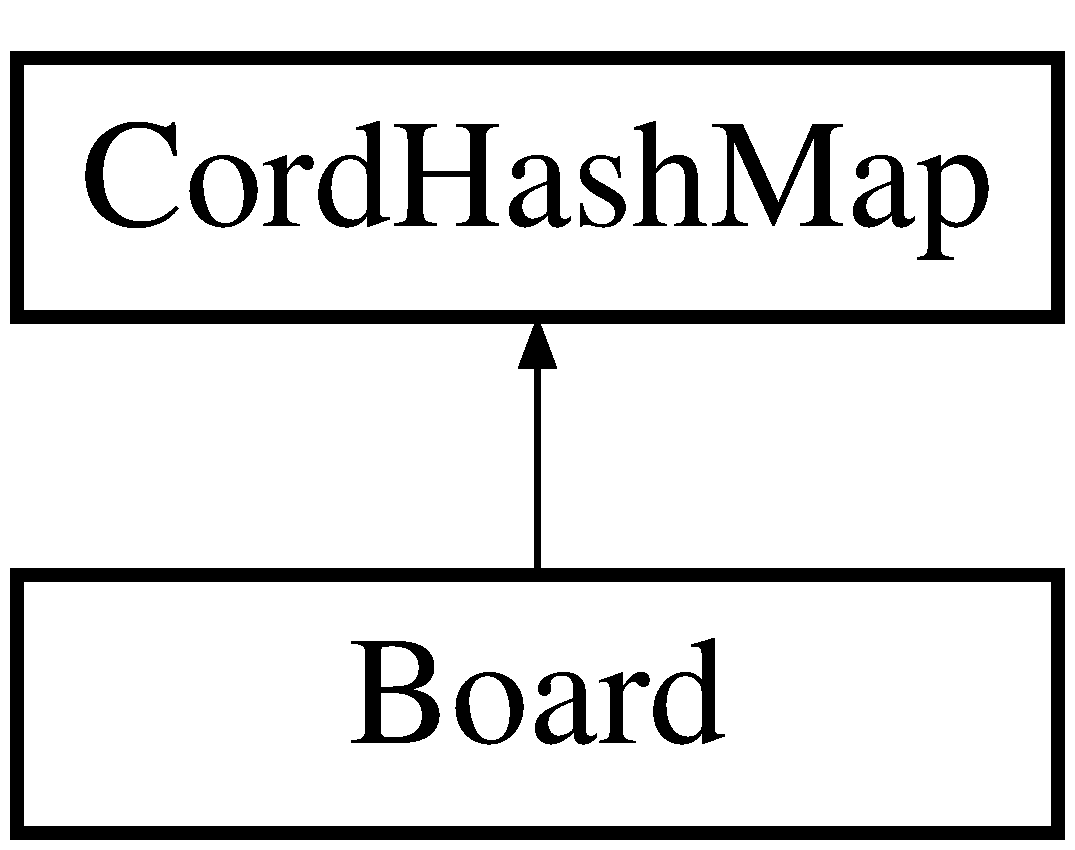
\includegraphics[height=2.000000cm]{class_board}
\end{center}
\end{figure}
\subsection*{Public Member Functions}
\begin{DoxyCompactItemize}
\item 
\hyperlink{class_board_a3b16444f12f23b4b4752b0a79ca4d295}{Board} (int size)
\end{DoxyCompactItemize}


\subsection{Detailed Description}
\hyperlink{_board_8java}{Board.\+java}

Author\+: Guthrie Price Date\+: 5/18/2015 Purpose\+: Basic implementation of a board for the memory puzzle 

\subsection{Constructor \& Destructor Documentation}
\hypertarget{class_board_a3b16444f12f23b4b4752b0a79ca4d295}{}\index{Board@{Board}!Board@{Board}}
\index{Board@{Board}!Board@{Board}}
\subsubsection[{Board}]{\setlength{\rightskip}{0pt plus 5cm}Board.\+Board (
\begin{DoxyParamCaption}
\item[{int}]{size}
\end{DoxyParamCaption}
)}\label{class_board_a3b16444f12f23b4b4752b0a79ca4d295}


The documentation for this class was generated from the following file\+:\begin{DoxyCompactItemize}
\item 
\hyperlink{_board_8java}{Board.\+java}\end{DoxyCompactItemize}

\hypertarget{class_card}{}\section{Card Class Reference}
\label{class_card}\index{Card@{Card}}
Inheritance diagram for Card\+:\begin{figure}[H]
\begin{center}
\leavevmode
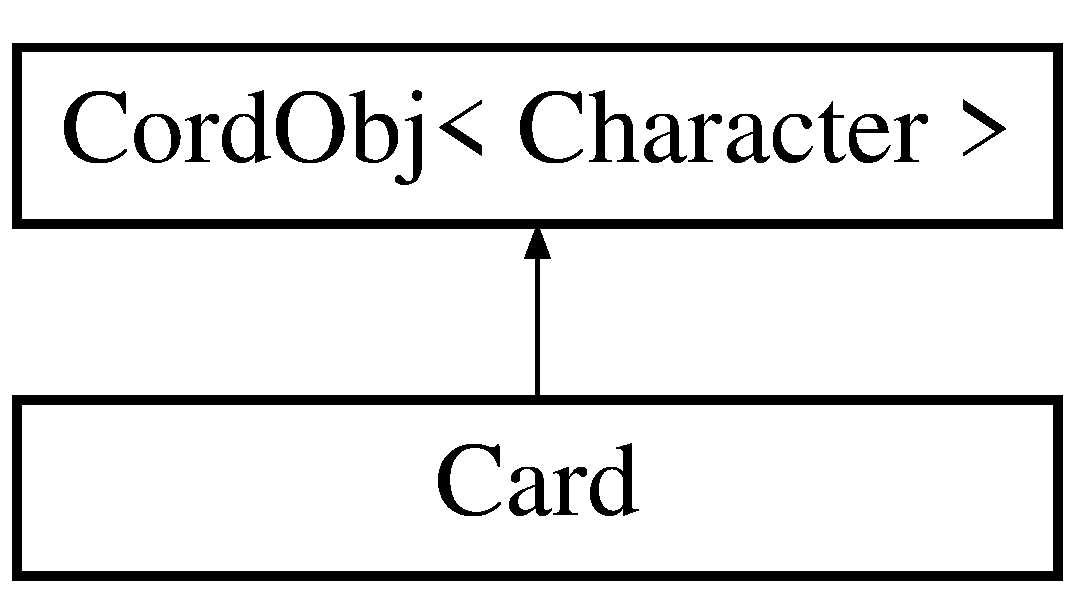
\includegraphics[height=2.000000cm]{class_card}
\end{center}
\end{figure}
\subsection*{Public Member Functions}
\begin{DoxyCompactItemize}
\item 
\hyperlink{class_card_a15ad9c9e7f3c9b4fede67eaaa2e485d4}{Card} (\hyperlink{class_coordinate}{Coordinate} cord, Character chr)
\item 
boolean \hyperlink{class_card_a3eaf46bc8f9c4df0c2018ba90dabb70a}{is\+Hidden} ()
\item 
void \hyperlink{class_card_a2ef0a0396f793a12076e968e471f68d0}{hide} ()
\item 
void \hyperlink{class_card_a28c61064054586bec26740f51900a82a}{show} ()
\item 
boolean \hyperlink{class_card_adbf03f9bcc93baf09641c66cbb78a9e7}{is\+Equal} (\hyperlink{class_card}{Card} card)
\end{DoxyCompactItemize}


\subsection{Detailed Description}
\hyperlink{_card_8java}{Card.\+java}

Author\+: Guthrie Price Date\+: 5/18/2015 Purpose\+: Represents a card for the memory puzzle 

\subsection{Constructor \& Destructor Documentation}
\hypertarget{class_card_a15ad9c9e7f3c9b4fede67eaaa2e485d4}{}\index{Card@{Card}!Card@{Card}}
\index{Card@{Card}!Card@{Card}}
\subsubsection[{Card}]{\setlength{\rightskip}{0pt plus 5cm}Card.\+Card (
\begin{DoxyParamCaption}
\item[{{\bf Coordinate}}]{cord, }
\item[{Character}]{chr}
\end{DoxyParamCaption}
)}\label{class_card_a15ad9c9e7f3c9b4fede67eaaa2e485d4}


\subsection{Member Function Documentation}
\hypertarget{class_card_a2ef0a0396f793a12076e968e471f68d0}{}\index{Card@{Card}!hide@{hide}}
\index{hide@{hide}!Card@{Card}}
\subsubsection[{hide}]{\setlength{\rightskip}{0pt plus 5cm}void Card.\+hide (
\begin{DoxyParamCaption}
{}
\end{DoxyParamCaption}
)}\label{class_card_a2ef0a0396f793a12076e968e471f68d0}
\hypertarget{class_card_adbf03f9bcc93baf09641c66cbb78a9e7}{}\index{Card@{Card}!is\+Equal@{is\+Equal}}
\index{is\+Equal@{is\+Equal}!Card@{Card}}
\subsubsection[{is\+Equal}]{\setlength{\rightskip}{0pt plus 5cm}boolean Card.\+is\+Equal (
\begin{DoxyParamCaption}
\item[{{\bf Card}}]{card}
\end{DoxyParamCaption}
)}\label{class_card_adbf03f9bcc93baf09641c66cbb78a9e7}
\hypertarget{class_card_a3eaf46bc8f9c4df0c2018ba90dabb70a}{}\index{Card@{Card}!is\+Hidden@{is\+Hidden}}
\index{is\+Hidden@{is\+Hidden}!Card@{Card}}
\subsubsection[{is\+Hidden}]{\setlength{\rightskip}{0pt plus 5cm}boolean Card.\+is\+Hidden (
\begin{DoxyParamCaption}
{}
\end{DoxyParamCaption}
)}\label{class_card_a3eaf46bc8f9c4df0c2018ba90dabb70a}
\hypertarget{class_card_a28c61064054586bec26740f51900a82a}{}\index{Card@{Card}!show@{show}}
\index{show@{show}!Card@{Card}}
\subsubsection[{show}]{\setlength{\rightskip}{0pt plus 5cm}void Card.\+show (
\begin{DoxyParamCaption}
{}
\end{DoxyParamCaption}
)}\label{class_card_a28c61064054586bec26740f51900a82a}


The documentation for this class was generated from the following file\+:\begin{DoxyCompactItemize}
\item 
\hyperlink{_card_8java}{Card.\+java}\end{DoxyCompactItemize}

\hypertarget{class_card_generator}{}\section{Card\+Generator Class Reference}
\label{class_card_generator}\index{Card\+Generator@{Card\+Generator}}
Inheritance diagram for Card\+Generator\+:\begin{figure}[H]
\begin{center}
\leavevmode
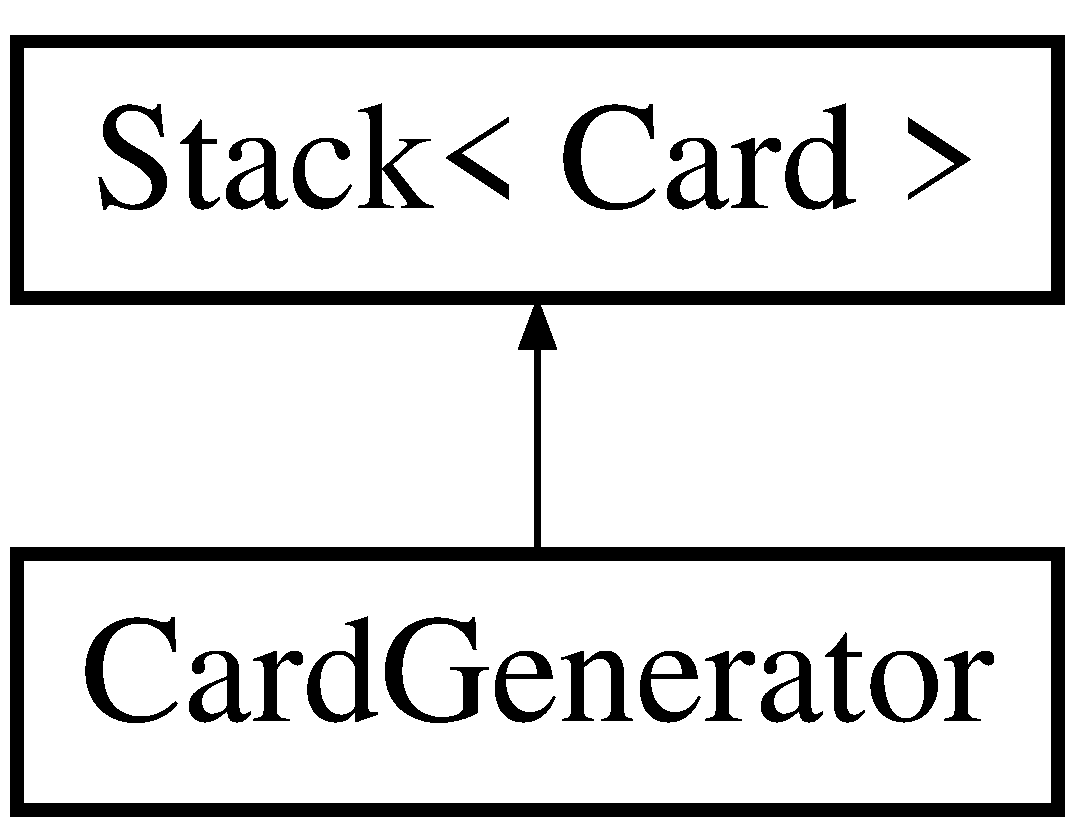
\includegraphics[height=2.000000cm]{class_card_generator}
\end{center}
\end{figure}
\subsection*{Public Member Functions}
\begin{DoxyCompactItemize}
\item 
\hyperlink{class_card_generator_afa8e0cfd8a8c1311a7ac79ccf26bee44}{Card\+Generator} (int size, char\mbox{[}$\,$\mbox{]} symbols)
\item 
void \hyperlink{class_card_generator_acd35f29f71013c383a16fb40cbd07341}{fill\+Stack} ()
\item 
void \hyperlink{class_card_generator_a126ec4afa79e9f27000416a40505d9e2}{set\+Space} (int size)
\item 
\hyperlink{class_card}{Card} \hyperlink{class_card_generator_ab7e34f991e3901c14b05ed1f4bd6f7a9}{get\+Rand\+Card} ()
\end{DoxyCompactItemize}
\subsection*{Additional Inherited Members}


\subsection{Constructor \& Destructor Documentation}
\hypertarget{class_card_generator_afa8e0cfd8a8c1311a7ac79ccf26bee44}{}\index{Card\+Generator@{Card\+Generator}!Card\+Generator@{Card\+Generator}}
\index{Card\+Generator@{Card\+Generator}!Card\+Generator@{Card\+Generator}}
\subsubsection[{Card\+Generator}]{\setlength{\rightskip}{0pt plus 5cm}Card\+Generator.\+Card\+Generator (
\begin{DoxyParamCaption}
\item[{int}]{size, }
\item[{char\mbox{[}$\,$\mbox{]}}]{symbols}
\end{DoxyParamCaption}
)}\label{class_card_generator_afa8e0cfd8a8c1311a7ac79ccf26bee44}


\subsection{Member Function Documentation}
\hypertarget{class_card_generator_acd35f29f71013c383a16fb40cbd07341}{}\index{Card\+Generator@{Card\+Generator}!fill\+Stack@{fill\+Stack}}
\index{fill\+Stack@{fill\+Stack}!Card\+Generator@{Card\+Generator}}
\subsubsection[{fill\+Stack}]{\setlength{\rightskip}{0pt plus 5cm}void Card\+Generator.\+fill\+Stack (
\begin{DoxyParamCaption}
{}
\end{DoxyParamCaption}
)}\label{class_card_generator_acd35f29f71013c383a16fb40cbd07341}
\hypertarget{class_card_generator_ab7e34f991e3901c14b05ed1f4bd6f7a9}{}\index{Card\+Generator@{Card\+Generator}!get\+Rand\+Card@{get\+Rand\+Card}}
\index{get\+Rand\+Card@{get\+Rand\+Card}!Card\+Generator@{Card\+Generator}}
\subsubsection[{get\+Rand\+Card}]{\setlength{\rightskip}{0pt plus 5cm}{\bf Card} Card\+Generator.\+get\+Rand\+Card (
\begin{DoxyParamCaption}
{}
\end{DoxyParamCaption}
)}\label{class_card_generator_ab7e34f991e3901c14b05ed1f4bd6f7a9}
\hypertarget{class_card_generator_a126ec4afa79e9f27000416a40505d9e2}{}\index{Card\+Generator@{Card\+Generator}!set\+Space@{set\+Space}}
\index{set\+Space@{set\+Space}!Card\+Generator@{Card\+Generator}}
\subsubsection[{set\+Space}]{\setlength{\rightskip}{0pt plus 5cm}void Card\+Generator.\+set\+Space (
\begin{DoxyParamCaption}
\item[{int}]{size}
\end{DoxyParamCaption}
)}\label{class_card_generator_a126ec4afa79e9f27000416a40505d9e2}


The documentation for this class was generated from the following file\+:\begin{DoxyCompactItemize}
\item 
\hyperlink{_card_generator_8java}{Card\+Generator.\+java}\end{DoxyCompactItemize}

\hypertarget{class_coordinate}{}\section{Coordinate Class Reference}
\label{class_coordinate}\index{Coordinate@{Coordinate}}
\subsection*{Public Member Functions}
\begin{DoxyCompactItemize}
\item 
\hyperlink{class_coordinate_a6ed2edfc96c9d825add1dfcdd923477d}{Coordinate} (Integer x\+Val, Integer y\+Val)
\item 
void \hyperlink{class_coordinate_a46811ded7b3fdefcf26d5eba99a24a26}{set\+X} (Integer x\+Val)
\item 
void \hyperlink{class_coordinate_a1259033f0f1dd22f12f7f126512bb3ff}{set\+Y} (Integer y\+Val)
\item 
Integer \hyperlink{class_coordinate_afb94c3f43076218846cef2fdd846d5f5}{get\+X} ()
\item 
Integer \hyperlink{class_coordinate_a6f9c9549760bf34732ba298461ea8b9b}{get\+Y} ()
\item 
boolean \hyperlink{class_coordinate_a6d24baa52c1cce49c0f14539e1316c8b}{is\+Equal} (\hyperlink{class_coordinate}{Coordinate} c)
\item 
String \hyperlink{class_coordinate_a539a31586fe7e7fca90a7bfb5118bb40}{to\+String} ()
\end{DoxyCompactItemize}


\subsection{Detailed Description}
\hyperlink{_coordinate_8java}{Coordinate.\+java}

Author\+: Guthrie Price Date\+: 5/18/2015 Purpose\+: A representation of a coordinate in a 2-\/dimensional space 

\subsection{Constructor \& Destructor Documentation}
\hypertarget{class_coordinate_a6ed2edfc96c9d825add1dfcdd923477d}{}\index{Coordinate@{Coordinate}!Coordinate@{Coordinate}}
\index{Coordinate@{Coordinate}!Coordinate@{Coordinate}}
\subsubsection[{Coordinate}]{\setlength{\rightskip}{0pt plus 5cm}Coordinate.\+Coordinate (
\begin{DoxyParamCaption}
\item[{Integer}]{x\+Val, }
\item[{Integer}]{y\+Val}
\end{DoxyParamCaption}
)}\label{class_coordinate_a6ed2edfc96c9d825add1dfcdd923477d}


\subsection{Member Function Documentation}
\hypertarget{class_coordinate_afb94c3f43076218846cef2fdd846d5f5}{}\index{Coordinate@{Coordinate}!get\+X@{get\+X}}
\index{get\+X@{get\+X}!Coordinate@{Coordinate}}
\subsubsection[{get\+X}]{\setlength{\rightskip}{0pt plus 5cm}Integer Coordinate.\+get\+X (
\begin{DoxyParamCaption}
{}
\end{DoxyParamCaption}
)}\label{class_coordinate_afb94c3f43076218846cef2fdd846d5f5}
\hypertarget{class_coordinate_a6f9c9549760bf34732ba298461ea8b9b}{}\index{Coordinate@{Coordinate}!get\+Y@{get\+Y}}
\index{get\+Y@{get\+Y}!Coordinate@{Coordinate}}
\subsubsection[{get\+Y}]{\setlength{\rightskip}{0pt plus 5cm}Integer Coordinate.\+get\+Y (
\begin{DoxyParamCaption}
{}
\end{DoxyParamCaption}
)}\label{class_coordinate_a6f9c9549760bf34732ba298461ea8b9b}
\hypertarget{class_coordinate_a6d24baa52c1cce49c0f14539e1316c8b}{}\index{Coordinate@{Coordinate}!is\+Equal@{is\+Equal}}
\index{is\+Equal@{is\+Equal}!Coordinate@{Coordinate}}
\subsubsection[{is\+Equal}]{\setlength{\rightskip}{0pt plus 5cm}boolean Coordinate.\+is\+Equal (
\begin{DoxyParamCaption}
\item[{{\bf Coordinate}}]{c}
\end{DoxyParamCaption}
)}\label{class_coordinate_a6d24baa52c1cce49c0f14539e1316c8b}
\hypertarget{class_coordinate_a46811ded7b3fdefcf26d5eba99a24a26}{}\index{Coordinate@{Coordinate}!set\+X@{set\+X}}
\index{set\+X@{set\+X}!Coordinate@{Coordinate}}
\subsubsection[{set\+X}]{\setlength{\rightskip}{0pt plus 5cm}void Coordinate.\+set\+X (
\begin{DoxyParamCaption}
\item[{Integer}]{x\+Val}
\end{DoxyParamCaption}
)}\label{class_coordinate_a46811ded7b3fdefcf26d5eba99a24a26}
\hypertarget{class_coordinate_a1259033f0f1dd22f12f7f126512bb3ff}{}\index{Coordinate@{Coordinate}!set\+Y@{set\+Y}}
\index{set\+Y@{set\+Y}!Coordinate@{Coordinate}}
\subsubsection[{set\+Y}]{\setlength{\rightskip}{0pt plus 5cm}void Coordinate.\+set\+Y (
\begin{DoxyParamCaption}
\item[{Integer}]{y\+Val}
\end{DoxyParamCaption}
)}\label{class_coordinate_a1259033f0f1dd22f12f7f126512bb3ff}
\hypertarget{class_coordinate_a539a31586fe7e7fca90a7bfb5118bb40}{}\index{Coordinate@{Coordinate}!to\+String@{to\+String}}
\index{to\+String@{to\+String}!Coordinate@{Coordinate}}
\subsubsection[{to\+String}]{\setlength{\rightskip}{0pt plus 5cm}String Coordinate.\+to\+String (
\begin{DoxyParamCaption}
{}
\end{DoxyParamCaption}
)}\label{class_coordinate_a539a31586fe7e7fca90a7bfb5118bb40}


The documentation for this class was generated from the following file\+:\begin{DoxyCompactItemize}
\item 
\hyperlink{_coordinate_8java}{Coordinate.\+java}\end{DoxyCompactItemize}

\hypertarget{class_cord_hash_map}{}\section{Cord\+Hash\+Map Class Reference}
\label{class_cord_hash_map}\index{Cord\+Hash\+Map@{Cord\+Hash\+Map}}
Inheritance diagram for Cord\+Hash\+Map\+:\begin{figure}[H]
\begin{center}
\leavevmode
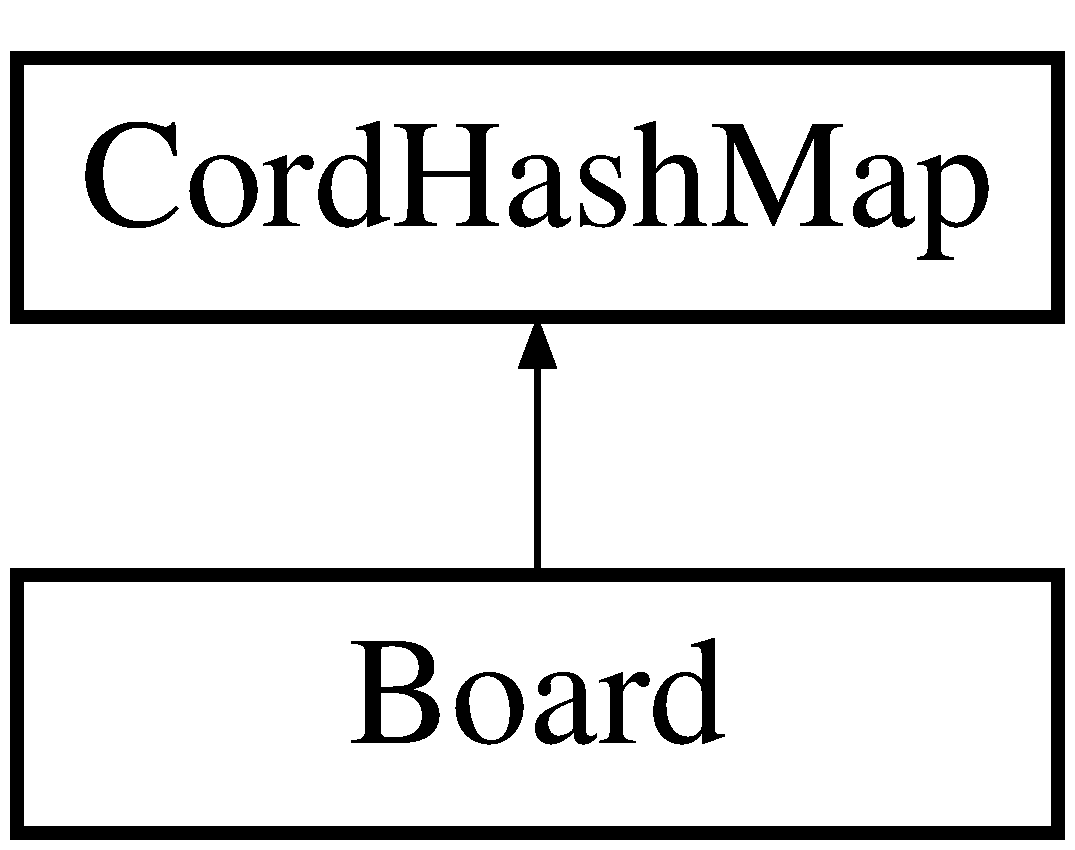
\includegraphics[height=2.000000cm]{class_cord_hash_map}
\end{center}
\end{figure}
\subsection*{Public Member Functions}
\begin{DoxyCompactItemize}
\item 
\hyperlink{class_cord_hash_map_a8b7beab76c8e2048d251941158be1c65}{Cord\+Hash\+Map} (int size)
\item 
\hyperlink{class_cord_obj}{Cord\+Obj}\mbox{[}$\,$\mbox{]} \hyperlink{class_cord_hash_map_a040e3766605a4ccc046da3fe813bc7b7}{get\+Space} ()
\item 
int \hyperlink{class_cord_hash_map_ae47e8b0916e228a6ddf5c47e12ed5af8}{get\+Size} ()
\item 
void \hyperlink{class_cord_hash_map_aed7b3f290de87054d8067f0ac8bd834a}{fill\+Space} (Vector$<$ \hyperlink{class_cord_obj}{Cord\+Obj} $>$ objs)
\item 
void \hyperlink{class_cord_hash_map_ae114ae6c105e744cb7fb3a2b8b64fe0e}{add} (\hyperlink{class_cord_obj}{Cord\+Obj} obj)
\item 
\hyperlink{class_cord_obj}{Cord\+Obj} \hyperlink{class_cord_hash_map_ac1ff06929ad693e358840a7ed9d18e04}{get} (\hyperlink{class_coordinate}{Coordinate} c)
\item 
int \hyperlink{class_cord_hash_map_aed7ac5b61130a6d79ab62d00a757d387}{hash} (\hyperlink{class_coordinate}{Coordinate} c)
\item 
String \hyperlink{class_cord_hash_map_a93265a3f480c90aa63616f37b5be9998}{to\+String} ()
\end{DoxyCompactItemize}


\subsection{Constructor \& Destructor Documentation}
\hypertarget{class_cord_hash_map_a8b7beab76c8e2048d251941158be1c65}{}\index{Cord\+Hash\+Map@{Cord\+Hash\+Map}!Cord\+Hash\+Map@{Cord\+Hash\+Map}}
\index{Cord\+Hash\+Map@{Cord\+Hash\+Map}!Cord\+Hash\+Map@{Cord\+Hash\+Map}}
\subsubsection[{Cord\+Hash\+Map}]{\setlength{\rightskip}{0pt plus 5cm}Cord\+Hash\+Map.\+Cord\+Hash\+Map (
\begin{DoxyParamCaption}
\item[{int}]{size}
\end{DoxyParamCaption}
)}\label{class_cord_hash_map_a8b7beab76c8e2048d251941158be1c65}


\subsection{Member Function Documentation}
\hypertarget{class_cord_hash_map_ae114ae6c105e744cb7fb3a2b8b64fe0e}{}\index{Cord\+Hash\+Map@{Cord\+Hash\+Map}!add@{add}}
\index{add@{add}!Cord\+Hash\+Map@{Cord\+Hash\+Map}}
\subsubsection[{add}]{\setlength{\rightskip}{0pt plus 5cm}void Cord\+Hash\+Map.\+add (
\begin{DoxyParamCaption}
\item[{{\bf Cord\+Obj}}]{obj}
\end{DoxyParamCaption}
)}\label{class_cord_hash_map_ae114ae6c105e744cb7fb3a2b8b64fe0e}
\hypertarget{class_cord_hash_map_aed7b3f290de87054d8067f0ac8bd834a}{}\index{Cord\+Hash\+Map@{Cord\+Hash\+Map}!fill\+Space@{fill\+Space}}
\index{fill\+Space@{fill\+Space}!Cord\+Hash\+Map@{Cord\+Hash\+Map}}
\subsubsection[{fill\+Space}]{\setlength{\rightskip}{0pt plus 5cm}void Cord\+Hash\+Map.\+fill\+Space (
\begin{DoxyParamCaption}
\item[{Vector$<$ {\bf Cord\+Obj} $>$}]{objs}
\end{DoxyParamCaption}
)}\label{class_cord_hash_map_aed7b3f290de87054d8067f0ac8bd834a}
\hypertarget{class_cord_hash_map_ac1ff06929ad693e358840a7ed9d18e04}{}\index{Cord\+Hash\+Map@{Cord\+Hash\+Map}!get@{get}}
\index{get@{get}!Cord\+Hash\+Map@{Cord\+Hash\+Map}}
\subsubsection[{get}]{\setlength{\rightskip}{0pt plus 5cm}{\bf Cord\+Obj} Cord\+Hash\+Map.\+get (
\begin{DoxyParamCaption}
\item[{{\bf Coordinate}}]{c}
\end{DoxyParamCaption}
)}\label{class_cord_hash_map_ac1ff06929ad693e358840a7ed9d18e04}
\hypertarget{class_cord_hash_map_ae47e8b0916e228a6ddf5c47e12ed5af8}{}\index{Cord\+Hash\+Map@{Cord\+Hash\+Map}!get\+Size@{get\+Size}}
\index{get\+Size@{get\+Size}!Cord\+Hash\+Map@{Cord\+Hash\+Map}}
\subsubsection[{get\+Size}]{\setlength{\rightskip}{0pt plus 5cm}int Cord\+Hash\+Map.\+get\+Size (
\begin{DoxyParamCaption}
{}
\end{DoxyParamCaption}
)}\label{class_cord_hash_map_ae47e8b0916e228a6ddf5c47e12ed5af8}
\hypertarget{class_cord_hash_map_a040e3766605a4ccc046da3fe813bc7b7}{}\index{Cord\+Hash\+Map@{Cord\+Hash\+Map}!get\+Space@{get\+Space}}
\index{get\+Space@{get\+Space}!Cord\+Hash\+Map@{Cord\+Hash\+Map}}
\subsubsection[{get\+Space}]{\setlength{\rightskip}{0pt plus 5cm}{\bf Cord\+Obj} \mbox{[}$\,$\mbox{]} Cord\+Hash\+Map.\+get\+Space (
\begin{DoxyParamCaption}
{}
\end{DoxyParamCaption}
)}\label{class_cord_hash_map_a040e3766605a4ccc046da3fe813bc7b7}
\hypertarget{class_cord_hash_map_aed7ac5b61130a6d79ab62d00a757d387}{}\index{Cord\+Hash\+Map@{Cord\+Hash\+Map}!hash@{hash}}
\index{hash@{hash}!Cord\+Hash\+Map@{Cord\+Hash\+Map}}
\subsubsection[{hash}]{\setlength{\rightskip}{0pt plus 5cm}int Cord\+Hash\+Map.\+hash (
\begin{DoxyParamCaption}
\item[{{\bf Coordinate}}]{c}
\end{DoxyParamCaption}
)}\label{class_cord_hash_map_aed7ac5b61130a6d79ab62d00a757d387}
\hypertarget{class_cord_hash_map_a93265a3f480c90aa63616f37b5be9998}{}\index{Cord\+Hash\+Map@{Cord\+Hash\+Map}!to\+String@{to\+String}}
\index{to\+String@{to\+String}!Cord\+Hash\+Map@{Cord\+Hash\+Map}}
\subsubsection[{to\+String}]{\setlength{\rightskip}{0pt plus 5cm}String Cord\+Hash\+Map.\+to\+String (
\begin{DoxyParamCaption}
{}
\end{DoxyParamCaption}
)}\label{class_cord_hash_map_a93265a3f480c90aa63616f37b5be9998}


The documentation for this class was generated from the following file\+:\begin{DoxyCompactItemize}
\item 
\hyperlink{_cord_hash_map_8java}{Cord\+Hash\+Map.\+java}\end{DoxyCompactItemize}

\hypertarget{class_cord_obj}{}\section{Cord\+Obj$<$ T $>$ Class Template Reference}
\label{class_cord_obj}\index{Cord\+Obj$<$ T $>$@{Cord\+Obj$<$ T $>$}}
\subsection*{Public Member Functions}
\begin{DoxyCompactItemize}
\item 
\hyperlink{class_cord_obj_a8bc54c06c2fd5ba119595e4a7185e594}{Cord\+Obj} (\hyperlink{class_coordinate}{Coordinate} c, T d)
\item 
\hyperlink{class_coordinate}{Coordinate} \hyperlink{class_cord_obj_a5bac352dcedaf6520c78b59259190f72}{get\+Cord} ()
\item 
T \hyperlink{class_cord_obj_a53c420550dd3fd3c9a2f57ca61cccc92}{get\+Data} ()
\item 
void \hyperlink{class_cord_obj_a5ddd79a158d348b3c687dc20eb82d487}{set\+Cord} (\hyperlink{class_coordinate}{Coordinate} c)
\item 
void \hyperlink{class_cord_obj_ab28e18954cd4fe1e3261db272b59c328}{set\+Data} (T d)
\item 
String \hyperlink{class_cord_obj_af7fc26f5dc62036e98c709a481376d87}{to\+String} ()
\end{DoxyCompactItemize}


\subsection{Detailed Description}
\hyperlink{_cord_obj_8java}{Cord\+Obj.\+java}

Author\+: Guthrie Price Date\+: 6/10/2015 Purpose\+: An abstract class for implmenting classes with data and a coordinate 

\subsection{Constructor \& Destructor Documentation}
\hypertarget{class_cord_obj_a8bc54c06c2fd5ba119595e4a7185e594}{}\index{Cord\+Obj@{Cord\+Obj}!Cord\+Obj@{Cord\+Obj}}
\index{Cord\+Obj@{Cord\+Obj}!Cord\+Obj@{Cord\+Obj}}
\subsubsection[{Cord\+Obj}]{\setlength{\rightskip}{0pt plus 5cm}{\bf Cord\+Obj}$<$ T $>$.{\bf Cord\+Obj} (
\begin{DoxyParamCaption}
\item[{{\bf Coordinate}}]{c, }
\item[{T}]{d}
\end{DoxyParamCaption}
)}\label{class_cord_obj_a8bc54c06c2fd5ba119595e4a7185e594}


\subsection{Member Function Documentation}
\hypertarget{class_cord_obj_a5bac352dcedaf6520c78b59259190f72}{}\index{Cord\+Obj@{Cord\+Obj}!get\+Cord@{get\+Cord}}
\index{get\+Cord@{get\+Cord}!Cord\+Obj@{Cord\+Obj}}
\subsubsection[{get\+Cord}]{\setlength{\rightskip}{0pt plus 5cm}{\bf Coordinate} {\bf Cord\+Obj}$<$ T $>$.get\+Cord (
\begin{DoxyParamCaption}
{}
\end{DoxyParamCaption}
)}\label{class_cord_obj_a5bac352dcedaf6520c78b59259190f72}
\hypertarget{class_cord_obj_a53c420550dd3fd3c9a2f57ca61cccc92}{}\index{Cord\+Obj@{Cord\+Obj}!get\+Data@{get\+Data}}
\index{get\+Data@{get\+Data}!Cord\+Obj@{Cord\+Obj}}
\subsubsection[{get\+Data}]{\setlength{\rightskip}{0pt plus 5cm}T {\bf Cord\+Obj}$<$ T $>$.get\+Data (
\begin{DoxyParamCaption}
{}
\end{DoxyParamCaption}
)}\label{class_cord_obj_a53c420550dd3fd3c9a2f57ca61cccc92}
\hypertarget{class_cord_obj_a5ddd79a158d348b3c687dc20eb82d487}{}\index{Cord\+Obj@{Cord\+Obj}!set\+Cord@{set\+Cord}}
\index{set\+Cord@{set\+Cord}!Cord\+Obj@{Cord\+Obj}}
\subsubsection[{set\+Cord}]{\setlength{\rightskip}{0pt plus 5cm}void {\bf Cord\+Obj}$<$ T $>$.set\+Cord (
\begin{DoxyParamCaption}
\item[{{\bf Coordinate}}]{c}
\end{DoxyParamCaption}
)}\label{class_cord_obj_a5ddd79a158d348b3c687dc20eb82d487}
\hypertarget{class_cord_obj_ab28e18954cd4fe1e3261db272b59c328}{}\index{Cord\+Obj@{Cord\+Obj}!set\+Data@{set\+Data}}
\index{set\+Data@{set\+Data}!Cord\+Obj@{Cord\+Obj}}
\subsubsection[{set\+Data}]{\setlength{\rightskip}{0pt plus 5cm}void {\bf Cord\+Obj}$<$ T $>$.set\+Data (
\begin{DoxyParamCaption}
\item[{T}]{d}
\end{DoxyParamCaption}
)}\label{class_cord_obj_ab28e18954cd4fe1e3261db272b59c328}
\hypertarget{class_cord_obj_af7fc26f5dc62036e98c709a481376d87}{}\index{Cord\+Obj@{Cord\+Obj}!to\+String@{to\+String}}
\index{to\+String@{to\+String}!Cord\+Obj@{Cord\+Obj}}
\subsubsection[{to\+String}]{\setlength{\rightskip}{0pt plus 5cm}String {\bf Cord\+Obj}$<$ T $>$.to\+String (
\begin{DoxyParamCaption}
{}
\end{DoxyParamCaption}
)}\label{class_cord_obj_af7fc26f5dc62036e98c709a481376d87}


The documentation for this class was generated from the following file\+:\begin{DoxyCompactItemize}
\item 
\hyperlink{_cord_obj_8java}{Cord\+Obj.\+java}\end{DoxyCompactItemize}

\hypertarget{class_driver}{}\section{Driver Class Reference}
\label{class_driver}\index{Driver@{Driver}}
\subsection*{Static Public Member Functions}
\begin{DoxyCompactItemize}
\item 
static void \hyperlink{class_driver_ad96bcac1144441cfe3fdf2e728349b79}{main} (String args\mbox{[}$\,$\mbox{]})
\end{DoxyCompactItemize}


\subsection{Member Function Documentation}
\hypertarget{class_driver_ad96bcac1144441cfe3fdf2e728349b79}{}\index{Driver@{Driver}!main@{main}}
\index{main@{main}!Driver@{Driver}}
\subsubsection[{main}]{\setlength{\rightskip}{0pt plus 5cm}static void Driver.\+main (
\begin{DoxyParamCaption}
\item[{String}]{args\mbox{[}$\,$\mbox{]}}
\end{DoxyParamCaption}
)\hspace{0.3cm}{\ttfamily [static]}}\label{class_driver_ad96bcac1144441cfe3fdf2e728349b79}


The documentation for this class was generated from the following file\+:\begin{DoxyCompactItemize}
\item 
\hyperlink{_driver_8java}{Driver.\+java}\end{DoxyCompactItemize}

\hypertarget{class_edge}{}\section{Edge Class Reference}
\label{class_edge}\index{Edge@{Edge}}
\subsection*{Public Member Functions}
\begin{DoxyCompactItemize}
\item 
\hyperlink{class_edge_a2a9b408174015f87b060fb2ac4d21f76}{Edge} (\hyperlink{class_vertex}{Vertex} start, \hyperlink{class_vertex}{Vertex} end, int w)
\item 
boolean \hyperlink{class_edge_a505ac8350db32e1270e87c5971aea7d2}{greater} (\hyperlink{class_edge}{Edge} e)
\end{DoxyCompactItemize}
\subsection*{Public Attributes}
\begin{DoxyCompactItemize}
\item 
\hyperlink{class_vertex}{Vertex} \hyperlink{class_edge_ad6c2f366711bc12a4b5cd7c113530b99}{v1}
\item 
\hyperlink{class_vertex}{Vertex} \hyperlink{class_edge_aa04d8e0773b9a6eb3708f8de7fb524aa}{v2}
\item 
int \hyperlink{class_edge_adcdae7ddae546193fe30e2a30e1ad53a}{weight}
\end{DoxyCompactItemize}


\subsection{Detailed Description}
\hyperlink{_edge_8java}{Edge.\+java}

Author\+: Guthrie Price 6/10/2015 Purpose\+: Class representing an undirected edge for the \hyperlink{class_graph}{Graph} class 

\subsection{Constructor \& Destructor Documentation}
\hypertarget{class_edge_a2a9b408174015f87b060fb2ac4d21f76}{}\index{Edge@{Edge}!Edge@{Edge}}
\index{Edge@{Edge}!Edge@{Edge}}
\subsubsection[{Edge}]{\setlength{\rightskip}{0pt plus 5cm}Edge.\+Edge (
\begin{DoxyParamCaption}
\item[{{\bf Vertex}}]{start, }
\item[{{\bf Vertex}}]{end, }
\item[{int}]{w}
\end{DoxyParamCaption}
)}\label{class_edge_a2a9b408174015f87b060fb2ac4d21f76}


\subsection{Member Function Documentation}
\hypertarget{class_edge_a505ac8350db32e1270e87c5971aea7d2}{}\index{Edge@{Edge}!greater@{greater}}
\index{greater@{greater}!Edge@{Edge}}
\subsubsection[{greater}]{\setlength{\rightskip}{0pt plus 5cm}boolean Edge.\+greater (
\begin{DoxyParamCaption}
\item[{{\bf Edge}}]{e}
\end{DoxyParamCaption}
)}\label{class_edge_a505ac8350db32e1270e87c5971aea7d2}


\subsection{Member Data Documentation}
\hypertarget{class_edge_ad6c2f366711bc12a4b5cd7c113530b99}{}\index{Edge@{Edge}!v1@{v1}}
\index{v1@{v1}!Edge@{Edge}}
\subsubsection[{v1}]{\setlength{\rightskip}{0pt plus 5cm}{\bf Vertex} Edge.\+v1}\label{class_edge_ad6c2f366711bc12a4b5cd7c113530b99}
\hypertarget{class_edge_aa04d8e0773b9a6eb3708f8de7fb524aa}{}\index{Edge@{Edge}!v2@{v2}}
\index{v2@{v2}!Edge@{Edge}}
\subsubsection[{v2}]{\setlength{\rightskip}{0pt plus 5cm}{\bf Vertex} Edge.\+v2}\label{class_edge_aa04d8e0773b9a6eb3708f8de7fb524aa}
\hypertarget{class_edge_adcdae7ddae546193fe30e2a30e1ad53a}{}\index{Edge@{Edge}!weight@{weight}}
\index{weight@{weight}!Edge@{Edge}}
\subsubsection[{weight}]{\setlength{\rightskip}{0pt plus 5cm}int Edge.\+weight}\label{class_edge_adcdae7ddae546193fe30e2a30e1ad53a}


The documentation for this class was generated from the following file\+:\begin{DoxyCompactItemize}
\item 
\hyperlink{_edge_8java}{Edge.\+java}\end{DoxyCompactItemize}

\hypertarget{class_graph}{}\section{Graph Class Reference}
\label{class_graph}\index{Graph@{Graph}}
\subsection*{Public Member Functions}
\begin{DoxyCompactItemize}
\item 
\hyperlink{class_graph_a3b41cdad7e5c5b479da2a4997b172ce1}{Graph} (int max\+Size)
\item 
\hyperlink{class_vertex}{Vertex}\mbox{[}$\,$\mbox{]} \hyperlink{class_graph_af46666375cb587dac0b9cb030c16a359}{get\+Vers} ()
\item 
int\mbox{[}$\,$\mbox{]}\mbox{[}$\,$\mbox{]} \hyperlink{class_graph_a252104f18213cb0f6e73487b26d22ef9}{get\+Edges} ()
\item 
void \hyperlink{class_graph_a9fa92fc6b57eb073390f5933689909df}{set\+Vers} (\hyperlink{class_vertex}{Vertex}\mbox{[}$\,$\mbox{]} vers)
\item 
void \hyperlink{class_graph_a0a5d1176c1e5096f098a1f49271270d3}{set\+Edges} (int\mbox{[}$\,$\mbox{]}\mbox{[}$\,$\mbox{]} edges)
\item 
int \hyperlink{class_graph_a3c51c040b54dfabf3f083f754928642f}{ver\+In\+Graph} (\hyperlink{class_vertex}{Vertex} v)
\item 
boolean \hyperlink{class_graph_ada66ac66d7a77f7a2b47ca33f7af5105}{add\+Vertex} (\hyperlink{class_vertex}{Vertex} v)
\item 
boolean \hyperlink{class_graph_a1d3e23f0b7be69dfcd3818e841cc6967}{add\+Edge} (\hyperlink{class_vertex}{Vertex} start, \hyperlink{class_vertex}{Vertex} end, int weight)
\item 
void \hyperlink{class_graph_aa58f9b45f4cd1b86169b7fc144175156}{connect} ()
\item 
void \hyperlink{class_graph_a00e73276d8291687bdfaf701ef32bb0c}{remove\+Edge} (\hyperlink{class_vertex}{Vertex} v1, \hyperlink{class_vertex}{Vertex} v2)
\item 
\hyperlink{class_graph}{Graph} \hyperlink{class_graph_a413b9997f5a2e850a78ad8f7aad89dab}{min\+Span\+Tree} ()
\item 
String \hyperlink{class_graph_a713307d8b2e43a9b717ca80f2d9fc8b0}{to\+String} ()
\end{DoxyCompactItemize}


\subsection{Constructor \& Destructor Documentation}
\hypertarget{class_graph_a3b41cdad7e5c5b479da2a4997b172ce1}{}\index{Graph@{Graph}!Graph@{Graph}}
\index{Graph@{Graph}!Graph@{Graph}}
\subsubsection[{Graph}]{\setlength{\rightskip}{0pt plus 5cm}Graph.\+Graph (
\begin{DoxyParamCaption}
\item[{int}]{max\+Size}
\end{DoxyParamCaption}
)}\label{class_graph_a3b41cdad7e5c5b479da2a4997b172ce1}


\subsection{Member Function Documentation}
\hypertarget{class_graph_a1d3e23f0b7be69dfcd3818e841cc6967}{}\index{Graph@{Graph}!add\+Edge@{add\+Edge}}
\index{add\+Edge@{add\+Edge}!Graph@{Graph}}
\subsubsection[{add\+Edge}]{\setlength{\rightskip}{0pt plus 5cm}boolean Graph.\+add\+Edge (
\begin{DoxyParamCaption}
\item[{{\bf Vertex}}]{start, }
\item[{{\bf Vertex}}]{end, }
\item[{int}]{weight}
\end{DoxyParamCaption}
)}\label{class_graph_a1d3e23f0b7be69dfcd3818e841cc6967}
\hypertarget{class_graph_ada66ac66d7a77f7a2b47ca33f7af5105}{}\index{Graph@{Graph}!add\+Vertex@{add\+Vertex}}
\index{add\+Vertex@{add\+Vertex}!Graph@{Graph}}
\subsubsection[{add\+Vertex}]{\setlength{\rightskip}{0pt plus 5cm}boolean Graph.\+add\+Vertex (
\begin{DoxyParamCaption}
\item[{{\bf Vertex}}]{v}
\end{DoxyParamCaption}
)}\label{class_graph_ada66ac66d7a77f7a2b47ca33f7af5105}
\hypertarget{class_graph_aa58f9b45f4cd1b86169b7fc144175156}{}\index{Graph@{Graph}!connect@{connect}}
\index{connect@{connect}!Graph@{Graph}}
\subsubsection[{connect}]{\setlength{\rightskip}{0pt plus 5cm}void Graph.\+connect (
\begin{DoxyParamCaption}
{}
\end{DoxyParamCaption}
)}\label{class_graph_aa58f9b45f4cd1b86169b7fc144175156}
\hypertarget{class_graph_a252104f18213cb0f6e73487b26d22ef9}{}\index{Graph@{Graph}!get\+Edges@{get\+Edges}}
\index{get\+Edges@{get\+Edges}!Graph@{Graph}}
\subsubsection[{get\+Edges}]{\setlength{\rightskip}{0pt plus 5cm}int \mbox{[}$\,$\mbox{]}\mbox{[}$\,$\mbox{]} Graph.\+get\+Edges (
\begin{DoxyParamCaption}
{}
\end{DoxyParamCaption}
)}\label{class_graph_a252104f18213cb0f6e73487b26d22ef9}
\hypertarget{class_graph_af46666375cb587dac0b9cb030c16a359}{}\index{Graph@{Graph}!get\+Vers@{get\+Vers}}
\index{get\+Vers@{get\+Vers}!Graph@{Graph}}
\subsubsection[{get\+Vers}]{\setlength{\rightskip}{0pt plus 5cm}{\bf Vertex} \mbox{[}$\,$\mbox{]} Graph.\+get\+Vers (
\begin{DoxyParamCaption}
{}
\end{DoxyParamCaption}
)}\label{class_graph_af46666375cb587dac0b9cb030c16a359}
\hypertarget{class_graph_a413b9997f5a2e850a78ad8f7aad89dab}{}\index{Graph@{Graph}!min\+Span\+Tree@{min\+Span\+Tree}}
\index{min\+Span\+Tree@{min\+Span\+Tree}!Graph@{Graph}}
\subsubsection[{min\+Span\+Tree}]{\setlength{\rightskip}{0pt plus 5cm}{\bf Graph} Graph.\+min\+Span\+Tree (
\begin{DoxyParamCaption}
{}
\end{DoxyParamCaption}
)}\label{class_graph_a413b9997f5a2e850a78ad8f7aad89dab}
\hypertarget{class_graph_a00e73276d8291687bdfaf701ef32bb0c}{}\index{Graph@{Graph}!remove\+Edge@{remove\+Edge}}
\index{remove\+Edge@{remove\+Edge}!Graph@{Graph}}
\subsubsection[{remove\+Edge}]{\setlength{\rightskip}{0pt plus 5cm}void Graph.\+remove\+Edge (
\begin{DoxyParamCaption}
\item[{{\bf Vertex}}]{v1, }
\item[{{\bf Vertex}}]{v2}
\end{DoxyParamCaption}
)}\label{class_graph_a00e73276d8291687bdfaf701ef32bb0c}
\hypertarget{class_graph_a0a5d1176c1e5096f098a1f49271270d3}{}\index{Graph@{Graph}!set\+Edges@{set\+Edges}}
\index{set\+Edges@{set\+Edges}!Graph@{Graph}}
\subsubsection[{set\+Edges}]{\setlength{\rightskip}{0pt plus 5cm}void Graph.\+set\+Edges (
\begin{DoxyParamCaption}
\item[{int}]{edges\mbox{[}$\,$\mbox{]}\mbox{[}$\,$\mbox{]}}
\end{DoxyParamCaption}
)}\label{class_graph_a0a5d1176c1e5096f098a1f49271270d3}
\hypertarget{class_graph_a9fa92fc6b57eb073390f5933689909df}{}\index{Graph@{Graph}!set\+Vers@{set\+Vers}}
\index{set\+Vers@{set\+Vers}!Graph@{Graph}}
\subsubsection[{set\+Vers}]{\setlength{\rightskip}{0pt plus 5cm}void Graph.\+set\+Vers (
\begin{DoxyParamCaption}
\item[{{\bf Vertex}\mbox{[}$\,$\mbox{]}}]{vers}
\end{DoxyParamCaption}
)}\label{class_graph_a9fa92fc6b57eb073390f5933689909df}
\hypertarget{class_graph_a713307d8b2e43a9b717ca80f2d9fc8b0}{}\index{Graph@{Graph}!to\+String@{to\+String}}
\index{to\+String@{to\+String}!Graph@{Graph}}
\subsubsection[{to\+String}]{\setlength{\rightskip}{0pt plus 5cm}String Graph.\+to\+String (
\begin{DoxyParamCaption}
{}
\end{DoxyParamCaption}
)}\label{class_graph_a713307d8b2e43a9b717ca80f2d9fc8b0}
\hypertarget{class_graph_a3c51c040b54dfabf3f083f754928642f}{}\index{Graph@{Graph}!ver\+In\+Graph@{ver\+In\+Graph}}
\index{ver\+In\+Graph@{ver\+In\+Graph}!Graph@{Graph}}
\subsubsection[{ver\+In\+Graph}]{\setlength{\rightskip}{0pt plus 5cm}int Graph.\+ver\+In\+Graph (
\begin{DoxyParamCaption}
\item[{{\bf Vertex}}]{v}
\end{DoxyParamCaption}
)}\label{class_graph_a3c51c040b54dfabf3f083f754928642f}


The documentation for this class was generated from the following file\+:\begin{DoxyCompactItemize}
\item 
\hyperlink{_graph_8java}{Graph.\+java}\end{DoxyCompactItemize}

\hypertarget{class_guessing_game}{}\section{Guessing\+Game Class Reference}
\label{class_guessing_game}\index{Guessing\+Game@{Guessing\+Game}}
\subsection*{Public Member Functions}
\begin{DoxyCompactItemize}
\item 
\hyperlink{class_guessing_game_a1c19223aceced88b73c81a5a7487577e}{Guessing\+Game} (Scanner input)
\item 
void \hyperlink{class_guessing_game_af56e7cf869802679f3dea5dd47ae4ea9}{run} ()
\end{DoxyCompactItemize}


\subsection{Constructor \& Destructor Documentation}
\hypertarget{class_guessing_game_a1c19223aceced88b73c81a5a7487577e}{}\index{Guessing\+Game@{Guessing\+Game}!Guessing\+Game@{Guessing\+Game}}
\index{Guessing\+Game@{Guessing\+Game}!Guessing\+Game@{Guessing\+Game}}
\subsubsection[{Guessing\+Game}]{\setlength{\rightskip}{0pt plus 5cm}Guessing\+Game.\+Guessing\+Game (
\begin{DoxyParamCaption}
\item[{Scanner}]{input}
\end{DoxyParamCaption}
)}\label{class_guessing_game_a1c19223aceced88b73c81a5a7487577e}


\subsection{Member Function Documentation}
\hypertarget{class_guessing_game_af56e7cf869802679f3dea5dd47ae4ea9}{}\index{Guessing\+Game@{Guessing\+Game}!run@{run}}
\index{run@{run}!Guessing\+Game@{Guessing\+Game}}
\subsubsection[{run}]{\setlength{\rightskip}{0pt plus 5cm}void Guessing\+Game.\+run (
\begin{DoxyParamCaption}
{}
\end{DoxyParamCaption}
)}\label{class_guessing_game_af56e7cf869802679f3dea5dd47ae4ea9}


The documentation for this class was generated from the following file\+:\begin{DoxyCompactItemize}
\item 
\hyperlink{_guessing_game_8java}{Guessing\+Game.\+java}\end{DoxyCompactItemize}

\hypertarget{class_linked_list}{}\section{Linked\+List$<$ T $>$ Class Template Reference}
\label{class_linked_list}\index{Linked\+List$<$ T $>$@{Linked\+List$<$ T $>$}}
\subsection*{Public Member Functions}
\begin{DoxyCompactItemize}
\item 
\hyperlink{class_linked_list_ae04bfb6ff80214a33132ba72ceb117aa}{Linked\+List} ()
\item 
void \hyperlink{class_linked_list_ae8784a0d7d68cdc679770f2f2fa1c6fc}{append} (T data)
\item 
void \hyperlink{class_linked_list_afce206a5ac36cd828efe7304cb1ab59f}{insert} (T data, int index)
\item 
boolean \hyperlink{class_linked_list_abcf20c4e8e87b09dd33f3b71d822c3cd}{remove} (int index)
\item 
T \hyperlink{class_linked_list_a032ef46fc54f12525746d9f7c3a80663}{get} (int index)
\item 
int \hyperlink{class_linked_list_aa01d8a9ebcc72b9d0abddaf5ba7d5d1a}{size} ()
\item 
String \hyperlink{class_linked_list_a7ddf314d6014b8227021cef8e054ae03}{to\+String} ()
\end{DoxyCompactItemize}


\subsection{Detailed Description}
\hyperlink{_linked_list_8java}{Linked\+List.\+java}

Author\+: Guthrie Price 3/16/2015 -\/ Data Structures (C\+S\+C-\/18\+C 42030) Implementation of a linked list. 

\subsection{Constructor \& Destructor Documentation}
\hypertarget{class_linked_list_ae04bfb6ff80214a33132ba72ceb117aa}{}\index{Linked\+List@{Linked\+List}!Linked\+List@{Linked\+List}}
\index{Linked\+List@{Linked\+List}!Linked\+List@{Linked\+List}}
\subsubsection[{Linked\+List}]{\setlength{\rightskip}{0pt plus 5cm}{\bf Linked\+List}$<$ T $>$.{\bf Linked\+List} (
\begin{DoxyParamCaption}
{}
\end{DoxyParamCaption}
)}\label{class_linked_list_ae04bfb6ff80214a33132ba72ceb117aa}


\subsection{Member Function Documentation}
\hypertarget{class_linked_list_ae8784a0d7d68cdc679770f2f2fa1c6fc}{}\index{Linked\+List@{Linked\+List}!append@{append}}
\index{append@{append}!Linked\+List@{Linked\+List}}
\subsubsection[{append}]{\setlength{\rightskip}{0pt plus 5cm}void {\bf Linked\+List}$<$ T $>$.append (
\begin{DoxyParamCaption}
\item[{T}]{data}
\end{DoxyParamCaption}
)}\label{class_linked_list_ae8784a0d7d68cdc679770f2f2fa1c6fc}
\hypertarget{class_linked_list_a032ef46fc54f12525746d9f7c3a80663}{}\index{Linked\+List@{Linked\+List}!get@{get}}
\index{get@{get}!Linked\+List@{Linked\+List}}
\subsubsection[{get}]{\setlength{\rightskip}{0pt plus 5cm}T {\bf Linked\+List}$<$ T $>$.get (
\begin{DoxyParamCaption}
\item[{int}]{index}
\end{DoxyParamCaption}
)}\label{class_linked_list_a032ef46fc54f12525746d9f7c3a80663}
\hypertarget{class_linked_list_afce206a5ac36cd828efe7304cb1ab59f}{}\index{Linked\+List@{Linked\+List}!insert@{insert}}
\index{insert@{insert}!Linked\+List@{Linked\+List}}
\subsubsection[{insert}]{\setlength{\rightskip}{0pt plus 5cm}void {\bf Linked\+List}$<$ T $>$.insert (
\begin{DoxyParamCaption}
\item[{T}]{data, }
\item[{int}]{index}
\end{DoxyParamCaption}
)}\label{class_linked_list_afce206a5ac36cd828efe7304cb1ab59f}
\hypertarget{class_linked_list_abcf20c4e8e87b09dd33f3b71d822c3cd}{}\index{Linked\+List@{Linked\+List}!remove@{remove}}
\index{remove@{remove}!Linked\+List@{Linked\+List}}
\subsubsection[{remove}]{\setlength{\rightskip}{0pt plus 5cm}boolean {\bf Linked\+List}$<$ T $>$.remove (
\begin{DoxyParamCaption}
\item[{int}]{index}
\end{DoxyParamCaption}
)}\label{class_linked_list_abcf20c4e8e87b09dd33f3b71d822c3cd}
\hypertarget{class_linked_list_aa01d8a9ebcc72b9d0abddaf5ba7d5d1a}{}\index{Linked\+List@{Linked\+List}!size@{size}}
\index{size@{size}!Linked\+List@{Linked\+List}}
\subsubsection[{size}]{\setlength{\rightskip}{0pt plus 5cm}int {\bf Linked\+List}$<$ T $>$.size (
\begin{DoxyParamCaption}
{}
\end{DoxyParamCaption}
)}\label{class_linked_list_aa01d8a9ebcc72b9d0abddaf5ba7d5d1a}
\hypertarget{class_linked_list_a7ddf314d6014b8227021cef8e054ae03}{}\index{Linked\+List@{Linked\+List}!to\+String@{to\+String}}
\index{to\+String@{to\+String}!Linked\+List@{Linked\+List}}
\subsubsection[{to\+String}]{\setlength{\rightskip}{0pt plus 5cm}String {\bf Linked\+List}$<$ T $>$.to\+String (
\begin{DoxyParamCaption}
{}
\end{DoxyParamCaption}
)}\label{class_linked_list_a7ddf314d6014b8227021cef8e054ae03}


The documentation for this class was generated from the following file\+:\begin{DoxyCompactItemize}
\item 
\hyperlink{_linked_list_8java}{Linked\+List.\+java}\end{DoxyCompactItemize}

\hypertarget{class_maze_game}{}\section{Maze\+Game Class Reference}
\label{class_maze_game}\index{Maze\+Game@{Maze\+Game}}
\subsection*{Public Member Functions}
\begin{DoxyCompactItemize}
\item 
\hyperlink{class_maze_game_a2f80d6e543b24c13fdf0338edd3841bb}{Maze\+Game} (int min\+Path, int dead\+Rooms, Scanner s)
\item 
void \hyperlink{class_maze_game_a2a2c681a1f1eab8b0073d6c18090dc8a}{run} ()
\item 
boolean \hyperlink{class_maze_game_ae89e6d9fe618350f59b58fdb12ecaecd}{game\+Over} (\hyperlink{class_vertex}{Vertex} current)
\item 
Array\+List$<$ Integer $>$ \hyperlink{class_maze_game_ae9037844dd5c02b5766ae32dda380c04}{output} (\hyperlink{class_vertex}{Vertex} cur\+Room)
\end{DoxyCompactItemize}


\subsection{Constructor \& Destructor Documentation}
\hypertarget{class_maze_game_a2f80d6e543b24c13fdf0338edd3841bb}{}\index{Maze\+Game@{Maze\+Game}!Maze\+Game@{Maze\+Game}}
\index{Maze\+Game@{Maze\+Game}!Maze\+Game@{Maze\+Game}}
\subsubsection[{Maze\+Game}]{\setlength{\rightskip}{0pt plus 5cm}Maze\+Game.\+Maze\+Game (
\begin{DoxyParamCaption}
\item[{int}]{min\+Path, }
\item[{int}]{dead\+Rooms, }
\item[{Scanner}]{s}
\end{DoxyParamCaption}
)}\label{class_maze_game_a2f80d6e543b24c13fdf0338edd3841bb}


\subsection{Member Function Documentation}
\hypertarget{class_maze_game_ae89e6d9fe618350f59b58fdb12ecaecd}{}\index{Maze\+Game@{Maze\+Game}!game\+Over@{game\+Over}}
\index{game\+Over@{game\+Over}!Maze\+Game@{Maze\+Game}}
\subsubsection[{game\+Over}]{\setlength{\rightskip}{0pt plus 5cm}boolean Maze\+Game.\+game\+Over (
\begin{DoxyParamCaption}
\item[{{\bf Vertex}}]{current}
\end{DoxyParamCaption}
)}\label{class_maze_game_ae89e6d9fe618350f59b58fdb12ecaecd}
\hypertarget{class_maze_game_ae9037844dd5c02b5766ae32dda380c04}{}\index{Maze\+Game@{Maze\+Game}!output@{output}}
\index{output@{output}!Maze\+Game@{Maze\+Game}}
\subsubsection[{output}]{\setlength{\rightskip}{0pt plus 5cm}Array\+List$<$Integer$>$ Maze\+Game.\+output (
\begin{DoxyParamCaption}
\item[{{\bf Vertex}}]{cur\+Room}
\end{DoxyParamCaption}
)}\label{class_maze_game_ae9037844dd5c02b5766ae32dda380c04}
\hypertarget{class_maze_game_a2a2c681a1f1eab8b0073d6c18090dc8a}{}\index{Maze\+Game@{Maze\+Game}!run@{run}}
\index{run@{run}!Maze\+Game@{Maze\+Game}}
\subsubsection[{run}]{\setlength{\rightskip}{0pt plus 5cm}void Maze\+Game.\+run (
\begin{DoxyParamCaption}
{}
\end{DoxyParamCaption}
)}\label{class_maze_game_a2a2c681a1f1eab8b0073d6c18090dc8a}


The documentation for this class was generated from the following file\+:\begin{DoxyCompactItemize}
\item 
\hyperlink{_maze_game_8java}{Maze\+Game.\+java}\end{DoxyCompactItemize}

\hypertarget{class_maze_generator}{}\section{Maze\+Generator Class Reference}
\label{class_maze_generator}\index{Maze\+Generator@{Maze\+Generator}}
\subsection*{Static Public Member Functions}
\begin{DoxyCompactItemize}
\item 
static \hyperlink{class_graph}{Graph} \hyperlink{class_maze_generator_a1bb75cefbd586dbbc77b13a1d65e620d}{generate\+Maze} (int min\+Path, int dead\+End)
\end{DoxyCompactItemize}


\subsection{Member Function Documentation}
\hypertarget{class_maze_generator_a1bb75cefbd586dbbc77b13a1d65e620d}{}\index{Maze\+Generator@{Maze\+Generator}!generate\+Maze@{generate\+Maze}}
\index{generate\+Maze@{generate\+Maze}!Maze\+Generator@{Maze\+Generator}}
\subsubsection[{generate\+Maze}]{\setlength{\rightskip}{0pt plus 5cm}static {\bf Graph} Maze\+Generator.\+generate\+Maze (
\begin{DoxyParamCaption}
\item[{int}]{min\+Path, }
\item[{int}]{dead\+End}
\end{DoxyParamCaption}
)\hspace{0.3cm}{\ttfamily [static]}}\label{class_maze_generator_a1bb75cefbd586dbbc77b13a1d65e620d}


The documentation for this class was generated from the following file\+:\begin{DoxyCompactItemize}
\item 
\hyperlink{_maze_generator_8java}{Maze\+Generator.\+java}\end{DoxyCompactItemize}

\hypertarget{class_memory_puzzle}{}\section{Memory\+Puzzle Class Reference}
\label{class_memory_puzzle}\index{Memory\+Puzzle@{Memory\+Puzzle}}
\subsection*{Public Member Functions}
\begin{DoxyCompactItemize}
\item 
\hyperlink{class_memory_puzzle_af0572c86f97440a7089e8557408d71ae}{Memory\+Puzzle} (char\mbox{[}$\,$\mbox{]} symbols, Scanner input)
\item 
void \hyperlink{class_memory_puzzle_a0a0b96db1eeb8d4a49ae81febb1d8171}{print\+Board} ()
\item 
\hyperlink{class_coordinate}{Coordinate} \hyperlink{class_memory_puzzle_a53a6329d54d8e90ccb966b9360454ec3}{get\+Cord} ()
\item 
boolean \hyperlink{class_memory_puzzle_af0d972cd2fc1c1076c76c7ba3cb20200}{game\+Over} (int guesses)
\item 
\hyperlink{class_card}{Card} \hyperlink{class_memory_puzzle_a5195289c677cbdde5f46b2f87ceafeb6}{get\+Card} ()
\item 
void \hyperlink{class_memory_puzzle_ab6b01c4fa2d3f4505e19276365147121}{print\+Main\+Menu} ()
\item 
boolean \hyperlink{class_memory_puzzle_a6ca2d7268d36c5a502436558138dc5ca}{valid\+Board\+Size} ()
\item 
void \hyperlink{class_memory_puzzle_a78a517d15a766e4b99dad52206a9c0d2}{run} ()
\item 
String \hyperlink{class_memory_puzzle_ace93b0f929bcb34f9dd9279b5a382432}{to\+String} ()
\end{DoxyCompactItemize}


\subsection{Constructor \& Destructor Documentation}
\hypertarget{class_memory_puzzle_af0572c86f97440a7089e8557408d71ae}{}\index{Memory\+Puzzle@{Memory\+Puzzle}!Memory\+Puzzle@{Memory\+Puzzle}}
\index{Memory\+Puzzle@{Memory\+Puzzle}!Memory\+Puzzle@{Memory\+Puzzle}}
\subsubsection[{Memory\+Puzzle}]{\setlength{\rightskip}{0pt plus 5cm}Memory\+Puzzle.\+Memory\+Puzzle (
\begin{DoxyParamCaption}
\item[{char\mbox{[}$\,$\mbox{]}}]{symbols, }
\item[{Scanner}]{input}
\end{DoxyParamCaption}
)}\label{class_memory_puzzle_af0572c86f97440a7089e8557408d71ae}


\subsection{Member Function Documentation}
\hypertarget{class_memory_puzzle_af0d972cd2fc1c1076c76c7ba3cb20200}{}\index{Memory\+Puzzle@{Memory\+Puzzle}!game\+Over@{game\+Over}}
\index{game\+Over@{game\+Over}!Memory\+Puzzle@{Memory\+Puzzle}}
\subsubsection[{game\+Over}]{\setlength{\rightskip}{0pt plus 5cm}boolean Memory\+Puzzle.\+game\+Over (
\begin{DoxyParamCaption}
\item[{int}]{guesses}
\end{DoxyParamCaption}
)}\label{class_memory_puzzle_af0d972cd2fc1c1076c76c7ba3cb20200}
\hypertarget{class_memory_puzzle_a5195289c677cbdde5f46b2f87ceafeb6}{}\index{Memory\+Puzzle@{Memory\+Puzzle}!get\+Card@{get\+Card}}
\index{get\+Card@{get\+Card}!Memory\+Puzzle@{Memory\+Puzzle}}
\subsubsection[{get\+Card}]{\setlength{\rightskip}{0pt plus 5cm}{\bf Card} Memory\+Puzzle.\+get\+Card (
\begin{DoxyParamCaption}
{}
\end{DoxyParamCaption}
)}\label{class_memory_puzzle_a5195289c677cbdde5f46b2f87ceafeb6}
\hypertarget{class_memory_puzzle_a53a6329d54d8e90ccb966b9360454ec3}{}\index{Memory\+Puzzle@{Memory\+Puzzle}!get\+Cord@{get\+Cord}}
\index{get\+Cord@{get\+Cord}!Memory\+Puzzle@{Memory\+Puzzle}}
\subsubsection[{get\+Cord}]{\setlength{\rightskip}{0pt plus 5cm}{\bf Coordinate} Memory\+Puzzle.\+get\+Cord (
\begin{DoxyParamCaption}
{}
\end{DoxyParamCaption}
)}\label{class_memory_puzzle_a53a6329d54d8e90ccb966b9360454ec3}
\hypertarget{class_memory_puzzle_a0a0b96db1eeb8d4a49ae81febb1d8171}{}\index{Memory\+Puzzle@{Memory\+Puzzle}!print\+Board@{print\+Board}}
\index{print\+Board@{print\+Board}!Memory\+Puzzle@{Memory\+Puzzle}}
\subsubsection[{print\+Board}]{\setlength{\rightskip}{0pt plus 5cm}void Memory\+Puzzle.\+print\+Board (
\begin{DoxyParamCaption}
{}
\end{DoxyParamCaption}
)}\label{class_memory_puzzle_a0a0b96db1eeb8d4a49ae81febb1d8171}
\hypertarget{class_memory_puzzle_ab6b01c4fa2d3f4505e19276365147121}{}\index{Memory\+Puzzle@{Memory\+Puzzle}!print\+Main\+Menu@{print\+Main\+Menu}}
\index{print\+Main\+Menu@{print\+Main\+Menu}!Memory\+Puzzle@{Memory\+Puzzle}}
\subsubsection[{print\+Main\+Menu}]{\setlength{\rightskip}{0pt plus 5cm}void Memory\+Puzzle.\+print\+Main\+Menu (
\begin{DoxyParamCaption}
{}
\end{DoxyParamCaption}
)}\label{class_memory_puzzle_ab6b01c4fa2d3f4505e19276365147121}
\hypertarget{class_memory_puzzle_a78a517d15a766e4b99dad52206a9c0d2}{}\index{Memory\+Puzzle@{Memory\+Puzzle}!run@{run}}
\index{run@{run}!Memory\+Puzzle@{Memory\+Puzzle}}
\subsubsection[{run}]{\setlength{\rightskip}{0pt plus 5cm}void Memory\+Puzzle.\+run (
\begin{DoxyParamCaption}
{}
\end{DoxyParamCaption}
)}\label{class_memory_puzzle_a78a517d15a766e4b99dad52206a9c0d2}
\hypertarget{class_memory_puzzle_ace93b0f929bcb34f9dd9279b5a382432}{}\index{Memory\+Puzzle@{Memory\+Puzzle}!to\+String@{to\+String}}
\index{to\+String@{to\+String}!Memory\+Puzzle@{Memory\+Puzzle}}
\subsubsection[{to\+String}]{\setlength{\rightskip}{0pt plus 5cm}String Memory\+Puzzle.\+to\+String (
\begin{DoxyParamCaption}
{}
\end{DoxyParamCaption}
)}\label{class_memory_puzzle_ace93b0f929bcb34f9dd9279b5a382432}
\hypertarget{class_memory_puzzle_a6ca2d7268d36c5a502436558138dc5ca}{}\index{Memory\+Puzzle@{Memory\+Puzzle}!valid\+Board\+Size@{valid\+Board\+Size}}
\index{valid\+Board\+Size@{valid\+Board\+Size}!Memory\+Puzzle@{Memory\+Puzzle}}
\subsubsection[{valid\+Board\+Size}]{\setlength{\rightskip}{0pt plus 5cm}boolean Memory\+Puzzle.\+valid\+Board\+Size (
\begin{DoxyParamCaption}
{}
\end{DoxyParamCaption}
)}\label{class_memory_puzzle_a6ca2d7268d36c5a502436558138dc5ca}


The documentation for this class was generated from the following file\+:\begin{DoxyCompactItemize}
\item 
\hyperlink{_memory_puzzle_8java}{Memory\+Puzzle.\+java}\end{DoxyCompactItemize}

\hypertarget{class_stack}{}\section{Stack$<$ T $>$ Class Template Reference}
\label{class_stack}\index{Stack$<$ T $>$@{Stack$<$ T $>$}}
\subsection*{Public Member Functions}
\begin{DoxyCompactItemize}
\item 
\hyperlink{class_stack_ae17728cf7d6856394c141d26dee8d3ac}{Stack} ()
\item 
void \hyperlink{class_stack_abb7eef0249d429b74486ab0063fc21c3}{push} (T data)
\item 
T \hyperlink{class_stack_a8c0776ba1b97449f3ed6c31035c983eb}{pop} ()
\item 
T \hyperlink{class_stack_a1789db27a750156f76be73551c4f1766}{peek} ()
\item 
boolean \hyperlink{class_stack_aba55fff63cbaec992328098cd21af7cf}{empty} ()
\item 
int \hyperlink{class_stack_af457b19c4596d16ed2392fa203b144d3}{size} ()
\item 
String \hyperlink{class_stack_a648cd7e04068ee38bb2ee45091d4c36b}{to\+String} ()
\end{DoxyCompactItemize}
\subsection*{Public Attributes}
\begin{DoxyCompactItemize}
\item 
\hyperlink{class_linked_list}{Linked\+List}$<$ T $>$ \hyperlink{class_stack_a3017fdb3715e4a0c8c81bdaa7c231a2c}{container}
\end{DoxyCompactItemize}


\subsection{Detailed Description}
\hyperlink{_stack_8java}{Stack.\+java}

Author\+: Guthrie Price 3/16/2015 -\/ Data Structures (C\+S\+C-\/18\+C 42030) Implementation of a stack using a linked list. 

\subsection{Constructor \& Destructor Documentation}
\hypertarget{class_stack_ae17728cf7d6856394c141d26dee8d3ac}{}\index{Stack@{Stack}!Stack@{Stack}}
\index{Stack@{Stack}!Stack@{Stack}}
\subsubsection[{Stack}]{\setlength{\rightskip}{0pt plus 5cm}{\bf Stack}$<$ T $>$.{\bf Stack} (
\begin{DoxyParamCaption}
{}
\end{DoxyParamCaption}
)}\label{class_stack_ae17728cf7d6856394c141d26dee8d3ac}


\subsection{Member Function Documentation}
\hypertarget{class_stack_aba55fff63cbaec992328098cd21af7cf}{}\index{Stack@{Stack}!empty@{empty}}
\index{empty@{empty}!Stack@{Stack}}
\subsubsection[{empty}]{\setlength{\rightskip}{0pt plus 5cm}boolean {\bf Stack}$<$ T $>$.empty (
\begin{DoxyParamCaption}
{}
\end{DoxyParamCaption}
)}\label{class_stack_aba55fff63cbaec992328098cd21af7cf}
\hypertarget{class_stack_a1789db27a750156f76be73551c4f1766}{}\index{Stack@{Stack}!peek@{peek}}
\index{peek@{peek}!Stack@{Stack}}
\subsubsection[{peek}]{\setlength{\rightskip}{0pt plus 5cm}T {\bf Stack}$<$ T $>$.peek (
\begin{DoxyParamCaption}
{}
\end{DoxyParamCaption}
)}\label{class_stack_a1789db27a750156f76be73551c4f1766}
\hypertarget{class_stack_a8c0776ba1b97449f3ed6c31035c983eb}{}\index{Stack@{Stack}!pop@{pop}}
\index{pop@{pop}!Stack@{Stack}}
\subsubsection[{pop}]{\setlength{\rightskip}{0pt plus 5cm}T {\bf Stack}$<$ T $>$.pop (
\begin{DoxyParamCaption}
{}
\end{DoxyParamCaption}
)}\label{class_stack_a8c0776ba1b97449f3ed6c31035c983eb}
\hypertarget{class_stack_abb7eef0249d429b74486ab0063fc21c3}{}\index{Stack@{Stack}!push@{push}}
\index{push@{push}!Stack@{Stack}}
\subsubsection[{push}]{\setlength{\rightskip}{0pt plus 5cm}void {\bf Stack}$<$ T $>$.push (
\begin{DoxyParamCaption}
\item[{T}]{data}
\end{DoxyParamCaption}
)}\label{class_stack_abb7eef0249d429b74486ab0063fc21c3}
\hypertarget{class_stack_af457b19c4596d16ed2392fa203b144d3}{}\index{Stack@{Stack}!size@{size}}
\index{size@{size}!Stack@{Stack}}
\subsubsection[{size}]{\setlength{\rightskip}{0pt plus 5cm}int {\bf Stack}$<$ T $>$.size (
\begin{DoxyParamCaption}
{}
\end{DoxyParamCaption}
)}\label{class_stack_af457b19c4596d16ed2392fa203b144d3}
\hypertarget{class_stack_a648cd7e04068ee38bb2ee45091d4c36b}{}\index{Stack@{Stack}!to\+String@{to\+String}}
\index{to\+String@{to\+String}!Stack@{Stack}}
\subsubsection[{to\+String}]{\setlength{\rightskip}{0pt plus 5cm}String {\bf Stack}$<$ T $>$.to\+String (
\begin{DoxyParamCaption}
{}
\end{DoxyParamCaption}
)}\label{class_stack_a648cd7e04068ee38bb2ee45091d4c36b}


\subsection{Member Data Documentation}
\hypertarget{class_stack_a3017fdb3715e4a0c8c81bdaa7c231a2c}{}\index{Stack@{Stack}!container@{container}}
\index{container@{container}!Stack@{Stack}}
\subsubsection[{container}]{\setlength{\rightskip}{0pt plus 5cm}{\bf Linked\+List}$<$T$>$ {\bf Stack}$<$ T $>$.container}\label{class_stack_a3017fdb3715e4a0c8c81bdaa7c231a2c}


The documentation for this class was generated from the following file\+:\begin{DoxyCompactItemize}
\item 
\hyperlink{_stack_8java}{Stack.\+java}\end{DoxyCompactItemize}

\hypertarget{class_utility}{}\section{Utility Class Reference}
\label{class_utility}\index{Utility@{Utility}}
\subsection*{Static Public Member Functions}
\begin{DoxyCompactItemize}
\item 
static int \hyperlink{class_utility_a569b78d6f68f09bfee365f3773cd4183}{pow} (int b, int a)
\item 
static int \hyperlink{class_utility_ab5ff7764f89dcf38e01bf189c684afbe}{get\+Number} (String prompt, int low\+Bnd, int up\+Bnd, Scanner input)
\item 
static void \hyperlink{class_utility_a694c1aebbf3d7b4efe0fd556a10283d6}{wait\+For\+Input} (Scanner input)
\item 
static void \hyperlink{class_utility_a2edbda8fa81e060b412aeb557a796fa3}{mrk\+Srt} (\hyperlink{class_edge}{Edge} a\mbox{[}$\,$\mbox{]})
\end{DoxyCompactItemize}


\subsection{Member Function Documentation}
\hypertarget{class_utility_ab5ff7764f89dcf38e01bf189c684afbe}{}\index{Utility@{Utility}!get\+Number@{get\+Number}}
\index{get\+Number@{get\+Number}!Utility@{Utility}}
\subsubsection[{get\+Number}]{\setlength{\rightskip}{0pt plus 5cm}static int Utility.\+get\+Number (
\begin{DoxyParamCaption}
\item[{String}]{prompt, }
\item[{int}]{low\+Bnd, }
\item[{int}]{up\+Bnd, }
\item[{Scanner}]{input}
\end{DoxyParamCaption}
)\hspace{0.3cm}{\ttfamily [static]}}\label{class_utility_ab5ff7764f89dcf38e01bf189c684afbe}
\hypertarget{class_utility_a2edbda8fa81e060b412aeb557a796fa3}{}\index{Utility@{Utility}!mrk\+Srt@{mrk\+Srt}}
\index{mrk\+Srt@{mrk\+Srt}!Utility@{Utility}}
\subsubsection[{mrk\+Srt}]{\setlength{\rightskip}{0pt plus 5cm}static void Utility.\+mrk\+Srt (
\begin{DoxyParamCaption}
\item[{{\bf Edge}}]{a\mbox{[}$\,$\mbox{]}}
\end{DoxyParamCaption}
)\hspace{0.3cm}{\ttfamily [static]}}\label{class_utility_a2edbda8fa81e060b412aeb557a796fa3}
\hypertarget{class_utility_a569b78d6f68f09bfee365f3773cd4183}{}\index{Utility@{Utility}!pow@{pow}}
\index{pow@{pow}!Utility@{Utility}}
\subsubsection[{pow}]{\setlength{\rightskip}{0pt plus 5cm}static int Utility.\+pow (
\begin{DoxyParamCaption}
\item[{int}]{b, }
\item[{int}]{a}
\end{DoxyParamCaption}
)\hspace{0.3cm}{\ttfamily [static]}}\label{class_utility_a569b78d6f68f09bfee365f3773cd4183}
\hypertarget{class_utility_a694c1aebbf3d7b4efe0fd556a10283d6}{}\index{Utility@{Utility}!wait\+For\+Input@{wait\+For\+Input}}
\index{wait\+For\+Input@{wait\+For\+Input}!Utility@{Utility}}
\subsubsection[{wait\+For\+Input}]{\setlength{\rightskip}{0pt plus 5cm}static void Utility.\+wait\+For\+Input (
\begin{DoxyParamCaption}
\item[{Scanner}]{input}
\end{DoxyParamCaption}
)\hspace{0.3cm}{\ttfamily [static]}}\label{class_utility_a694c1aebbf3d7b4efe0fd556a10283d6}


The documentation for this class was generated from the following file\+:\begin{DoxyCompactItemize}
\item 
\hyperlink{_utility_8java}{Utility.\+java}\end{DoxyCompactItemize}

\hypertarget{class_vertex}{}\section{Vertex Class Reference}
\label{class_vertex}\index{Vertex@{Vertex}}
\subsection*{Public Member Functions}
\begin{DoxyCompactItemize}
\item 
\hyperlink{class_vertex_a9c42dd2eb393748dc6c247a331859749}{Vertex} (int label)
\item 
boolean \hyperlink{class_vertex_a45f1191d2c089073be57f1df01eff15e}{equal} (\hyperlink{class_vertex}{Vertex} v)
\end{DoxyCompactItemize}


\subsection{Detailed Description}
\hyperlink{_vertex_8java}{Vertex.\+java}

Author\+: Guthrie Price 6/10/2015 Purpose\+: Class that represents a vertex in a graph 

\subsection{Constructor \& Destructor Documentation}
\hypertarget{class_vertex_a9c42dd2eb393748dc6c247a331859749}{}\index{Vertex@{Vertex}!Vertex@{Vertex}}
\index{Vertex@{Vertex}!Vertex@{Vertex}}
\subsubsection[{Vertex}]{\setlength{\rightskip}{0pt plus 5cm}Vertex.\+Vertex (
\begin{DoxyParamCaption}
\item[{int}]{label}
\end{DoxyParamCaption}
)}\label{class_vertex_a9c42dd2eb393748dc6c247a331859749}


\subsection{Member Function Documentation}
\hypertarget{class_vertex_a45f1191d2c089073be57f1df01eff15e}{}\index{Vertex@{Vertex}!equal@{equal}}
\index{equal@{equal}!Vertex@{Vertex}}
\subsubsection[{equal}]{\setlength{\rightskip}{0pt plus 5cm}boolean Vertex.\+equal (
\begin{DoxyParamCaption}
\item[{{\bf Vertex}}]{v}
\end{DoxyParamCaption}
)}\label{class_vertex_a45f1191d2c089073be57f1df01eff15e}


The documentation for this class was generated from the following file\+:\begin{DoxyCompactItemize}
\item 
\hyperlink{_vertex_8java}{Vertex.\+java}\end{DoxyCompactItemize}

\chapter{File Documentation}
\hypertarget{_a_v_l_node_8java}{}\section{A\+V\+L\+Node.\+java File Reference}
\label{_a_v_l_node_8java}\index{A\+V\+L\+Node.\+java@{A\+V\+L\+Node.\+java}}
\subsection*{Classes}
\begin{DoxyCompactItemize}
\item 
class \hyperlink{class_a_v_l_node}{A\+V\+L\+Node}
\end{DoxyCompactItemize}

\hypertarget{_a_v_l_tree_8java}{}\section{A\+V\+L\+Tree.\+java File Reference}
\label{_a_v_l_tree_8java}\index{A\+V\+L\+Tree.\+java@{A\+V\+L\+Tree.\+java}}
\subsection*{Classes}
\begin{DoxyCompactItemize}
\item 
class \hyperlink{class_a_v_l_tree}{A\+V\+L\+Tree}
\end{DoxyCompactItemize}

\hypertarget{_board_8java}{}\section{Board.\+java File Reference}
\label{_board_8java}\index{Board.\+java@{Board.\+java}}
\subsection*{Classes}
\begin{DoxyCompactItemize}
\item 
class \hyperlink{class_board}{Board}
\end{DoxyCompactItemize}

\hypertarget{_card_8java}{}\section{Card.\+java File Reference}
\label{_card_8java}\index{Card.\+java@{Card.\+java}}
\subsection*{Classes}
\begin{DoxyCompactItemize}
\item 
class \hyperlink{class_card}{Card}
\end{DoxyCompactItemize}

\hypertarget{_card_generator_8java}{}\section{Card\+Generator.\+java File Reference}
\label{_card_generator_8java}\index{Card\+Generator.\+java@{Card\+Generator.\+java}}
\subsection*{Classes}
\begin{DoxyCompactItemize}
\item 
class \hyperlink{class_card_generator}{Card\+Generator}
\end{DoxyCompactItemize}

\hypertarget{_coordinate_8java}{}\section{Coordinate.\+java File Reference}
\label{_coordinate_8java}\index{Coordinate.\+java@{Coordinate.\+java}}
\subsection*{Classes}
\begin{DoxyCompactItemize}
\item 
class \hyperlink{class_coordinate}{Coordinate}
\end{DoxyCompactItemize}

\hypertarget{_cord_hash_map_8java}{}\section{Cord\+Hash\+Map.\+java File Reference}
\label{_cord_hash_map_8java}\index{Cord\+Hash\+Map.\+java@{Cord\+Hash\+Map.\+java}}
\subsection*{Classes}
\begin{DoxyCompactItemize}
\item 
class \hyperlink{class_cord_hash_map}{Cord\+Hash\+Map}
\end{DoxyCompactItemize}

\hypertarget{_cord_obj_8java}{}\section{Cord\+Obj.\+java File Reference}
\label{_cord_obj_8java}\index{Cord\+Obj.\+java@{Cord\+Obj.\+java}}
\subsection*{Classes}
\begin{DoxyCompactItemize}
\item 
class \hyperlink{class_cord_obj}{Cord\+Obj$<$ T $>$}
\end{DoxyCompactItemize}

\hypertarget{_driver_8java}{}\section{Driver.\+java File Reference}
\label{_driver_8java}\index{Driver.\+java@{Driver.\+java}}
\subsection*{Classes}
\begin{DoxyCompactItemize}
\item 
class \hyperlink{class_driver}{Driver}
\end{DoxyCompactItemize}

\hypertarget{_edge_8java}{}\section{Edge.\+java File Reference}
\label{_edge_8java}\index{Edge.\+java@{Edge.\+java}}
\subsection*{Classes}
\begin{DoxyCompactItemize}
\item 
class \hyperlink{class_edge}{Edge}
\end{DoxyCompactItemize}

\hypertarget{_graph_8java}{}\section{Graph.\+java File Reference}
\label{_graph_8java}\index{Graph.\+java@{Graph.\+java}}
\subsection*{Classes}
\begin{DoxyCompactItemize}
\item 
class \hyperlink{class_graph}{Graph}
\end{DoxyCompactItemize}

\hypertarget{_guessing_game_8java}{}\section{Guessing\+Game.\+java File Reference}
\label{_guessing_game_8java}\index{Guessing\+Game.\+java@{Guessing\+Game.\+java}}
\subsection*{Classes}
\begin{DoxyCompactItemize}
\item 
class \hyperlink{class_guessing_game}{Guessing\+Game}
\end{DoxyCompactItemize}

\hypertarget{_linked_list_8java}{}\section{Linked\+List.\+java File Reference}
\label{_linked_list_8java}\index{Linked\+List.\+java@{Linked\+List.\+java}}
\subsection*{Classes}
\begin{DoxyCompactItemize}
\item 
class \hyperlink{class_linked_list}{Linked\+List$<$ T $>$}
\end{DoxyCompactItemize}

\hypertarget{_maze_game_8java}{}\section{Maze\+Game.\+java File Reference}
\label{_maze_game_8java}\index{Maze\+Game.\+java@{Maze\+Game.\+java}}
\subsection*{Classes}
\begin{DoxyCompactItemize}
\item 
class \hyperlink{class_maze_game}{Maze\+Game}
\end{DoxyCompactItemize}

\hypertarget{_maze_generator_8java}{}\section{Maze\+Generator.\+java File Reference}
\label{_maze_generator_8java}\index{Maze\+Generator.\+java@{Maze\+Generator.\+java}}
\subsection*{Classes}
\begin{DoxyCompactItemize}
\item 
class \hyperlink{class_maze_generator}{Maze\+Generator}
\end{DoxyCompactItemize}

\hypertarget{_memory_puzzle_8java}{}\section{Memory\+Puzzle.\+java File Reference}
\label{_memory_puzzle_8java}\index{Memory\+Puzzle.\+java@{Memory\+Puzzle.\+java}}
\subsection*{Classes}
\begin{DoxyCompactItemize}
\item 
class \hyperlink{class_memory_puzzle}{Memory\+Puzzle}
\end{DoxyCompactItemize}

\hypertarget{_stack_8java}{}\section{Stack.\+java File Reference}
\label{_stack_8java}\index{Stack.\+java@{Stack.\+java}}
\subsection*{Classes}
\begin{DoxyCompactItemize}
\item 
class \hyperlink{class_stack}{Stack$<$ T $>$}
\end{DoxyCompactItemize}

\hypertarget{_utility_8java}{}\section{Utility.\+java File Reference}
\label{_utility_8java}\index{Utility.\+java@{Utility.\+java}}
\subsection*{Classes}
\begin{DoxyCompactItemize}
\item 
class \hyperlink{class_utility}{Utility}
\end{DoxyCompactItemize}

\hypertarget{_vertex_8java}{}\section{Vertex.\+java File Reference}
\label{_vertex_8java}\index{Vertex.\+java@{Vertex.\+java}}
\subsection*{Classes}
\begin{DoxyCompactItemize}
\item 
class \hyperlink{class_vertex}{Vertex}
\end{DoxyCompactItemize}

%--- End generated contents ---

% Index
\backmatter
\newpage
\phantomsection
\clearemptydoublepage
\addcontentsline{toc}{chapter}{Index}
\printindex

\end{document}
